\documentclass[11pt]{article}

\usepackage[margin=1in]{geometry}
\usepackage{amsmath,amssymb}
\usepackage{bm}
\usepackage{booktabs}
\usepackage{enumitem}
\usepackage{algorithm}
\usepackage{algpseudocode}
\usepackage{hyperref}
\usepackage{xcolor}
\usepackage{tikz}
\usepackage{graphicx}
\usetikzlibrary{arrows.meta,positioning,decorations.pathreplacing}
\emergencystretch=1em

\definecolor{tealeafNavy}{HTML}{17324D}
\definecolor{tealeafTeal}{HTML}{168C8C}
\definecolor{tealeafLightTeal}{HTML}{DDF1EF}
\definecolor{tealeafOrange}{HTML}{E6813B}
\definecolor{tealeafLight}{HTML}{F3F6F7}

\newcommand{\expit}{\operatorname{expit}}
\newcommand{\logit}{\operatorname{logit}}
\newcommand{\BetaDist}{\operatorname{Beta}}

\title{Tealeaf: Testing Exon Alternatives Locally in Exon-Anchored Frames}
\author{}
\date{}

\begin{document}
\maketitle

\section{Introduction}

Differential splicing between cell types in single-cell RNA-seq is usually tested at one of three levels. Event methods (SUPPA2, rMATS) test predefined event types such as a skipped exon or an alternative 3' site. Junction methods (LeafCutter, scQuint, MAJIQ) test the relative use of junctions that share a splice site or exon, using junction-spanning reads (MAJIQ also intron-retention reads). Isoform methods estimate full-length transcript abundances, which short reads with strong positional bias identify poorly when transcripts differ at several distant sites. Tealeaf tests a different unit, the \emph{local splice path}, and adds the following.
\begin{enumerate}[leftmargin=*]
  \item \textbf{Local splice paths.} A splice block is a region of a gene between two constitutive exons, and its paths are all exon chains that transcripts take through it. A path set represents any local pattern, including several adjacent alternative exons, mutually exclusive exons, combinations of alternative splice sites and alternative first or last exons, in one test, without classifying it into event types. Because the rest of each transcript does not enter, a block has few paths that differ within a short window, so path usage is identifiable from short reads where full isoforms are not.
  \item \textbf{All reads in the block.} Every molecule overlapping the block contributes through the set of paths it is compatible with, including exon-body and unspliced reads, weighted by the number of read positions on each path that produce its class. Junction counts alone discard these reads. Where positional capture bias dominates exon-body coverage, at alternative transcript ends, the test uses junction-spanning molecules only.
  \item \textbf{Both primers.} Parse libraries prime each cell with poly(dT) and random hexamers, which sample transcripts with different positional bias. Both primers enter one likelihood with a primer offset estimated without cell-type labels, instead of pooling the primers or using one.
  \item \textbf{Unannotated paths.} Junction support counted over all cells, and therefore blind to cell-type labels, adds novel paths (alternative splice sites, new exons, novel first and last exons) and new blocks, which are tested with the same model as annotated paths.
  \item \textbf{Subjects as replicates.} A Beta--logit-normal model with a subject random intercept pairs the two cell types of each subject and allows extra variation between subject--cell-type rows. Count simulations under the null on the real designs show the tests are calibrated.
  \item \textbf{A self-contained implementation.} A targeted two-pass spliced aligner, with a compiled Rust kernel and FASTQ reader, reproduces STAR's alignment scoring and filters on the target genes and replaces whole-genome search for competing alignments by a genome-wide k-mer uniqueness table. Tealeaf runs from FASTQ files to tests without an external aligner or pseudoaligner; a run of 345 million read pairs aligns in about the time STARsolo takes, and the stored alignments of a run take about 1~GB instead of a 46~GB BAM file.
\end{enumerate}
On a mouse brain dataset of 48 subjects, Tealeaf replicates more genes across independent halves of the subjects than LeafCutter, MAJIQ, SUPPA2, primer-aware SUPPA2, rMATS and scQuint, on each method's own set of testable genes, and its top-ranked directions agree with independent single-cell long-read data as often as those of the best of these methods, over many more evaluable tests (Section~\ref{sec:evaluation}).

\section{Overview}

Tealeaf (Testing Exon Alternatives Locally in Exon-Anchored Frames) tests whether the usage of local splice paths differs between two cell types measured in the same subjects. The unit of analysis is a \emph{splice block}, a genomic window of one gene bounded by constitutive exons, the exon-anchored frame, in which transcripts take two or more alternative exon chains, the \emph{paths}. For every block and pair of cell types, Tealeaf asks whether the probability that a molecule from the block originates from a given path differs between the cell types, with subjects as biological replicates.

The method works from sequencing reads to tests in five steps (Figure~\ref{fig:pipeline}).
\begin{enumerate}[leftmargin=*]
  \item \textbf{Targeted spliced alignment.} Reads are aligned to the genomic loci of the target genes only, by an aligner that reproduces the scoring, filters and uniqueness criteria of a genome alignment with STAR, but replaces whole-genome search by a genome-wide k-mer uniqueness table. Alignment runs in two passes; the second uses splice junctions discovered in the first.
  \item \textbf{Blocks and paths.} Annotated splice blocks provide the annotated paths. Unannotated splice junctions, with support counted over all cells and therefore blind to cell-type labels, add novel paths (alternative splice sites, new exons, novel first and last exons) and new blocks.
  \item \textbf{Molecule classes.} Each UMI molecule that overlaps a block is assigned the set of paths it is compatible with, using only the parts of its reads inside the block window. Counts are tabulated by subject, cell type, primer (poly(dT) or random hexamer) and compatibility class.
  \item \textbf{Read opportunities.} For each path and class, the number of read start positions on the path that would produce that class gives the class probabilities as a function of path usage.
  \item \textbf{Test.} A Beta--logit-normal model with a subject random intercept and a primer offset is fitted to the class counts, each path is tested against the others by a likelihood-ratio test, and the path tests are combined by Simes' method.
\end{enumerate}
Blocks are split by their annotated structure. \emph{Internal} blocks, where all annotated paths share the first and last exon, use all reads that overlap the block. \emph{Terminal} blocks, which have alternative first or last exons or transcript ends, use only molecules that span a junction distinguishing the paths, because their exon-body coverage is dominated by the positional capture bias of the primers.

\begin{figure}[ht]
\centering
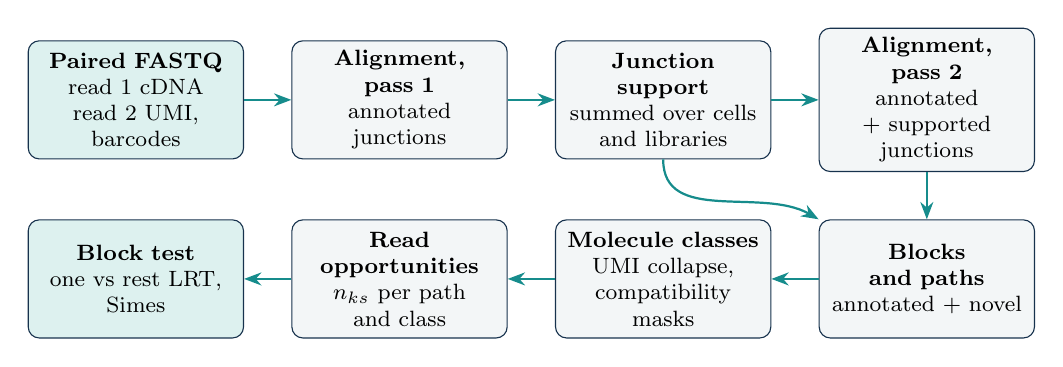
\begin{tikzpicture}[
  stage/.style={draw=tealeafNavy,rounded corners,fill=tealeafLight,align=center,font=\footnotesize,text width=25mm,minimum height=15mm},
  flow/.style={-{Stealth[length=2.2mm]},thick,draw=tealeafTeal},
  node distance=6mm and 6mm]
\node[stage,fill=tealeafLightTeal] (fastq) {\textbf{Paired FASTQ}\\read 1 cDNA\\read 2 UMI, barcodes};
\node[stage,right=of fastq] (pass1) {\textbf{Alignment, pass 1}\\annotated junctions};
\node[stage,right=of pass1] (junc) {\textbf{Junction support}\\summed over cells\\and libraries};
\node[stage,right=of junc] (pass2) {\textbf{Alignment, pass 2}\\annotated + supported\\junctions};
\node[stage,below=of pass2] (blocks) {\textbf{Blocks and paths}\\annotated + novel};
\node[stage,left=of blocks] (classes) {\textbf{Molecule classes}\\UMI collapse,\\compatibility masks};
\node[stage,left=of classes] (opps) {\textbf{Read}\\\textbf{opportunities}\\$n_{ks}$ per path and class};
\node[stage,left=of opps,fill=tealeafLightTeal] (test) {\textbf{Block test}\\one vs rest LRT,\\Simes};
\draw[flow] (fastq)--(pass1);
\draw[flow] (pass1)--(junc);
\draw[flow] (junc)--(pass2);
\draw[flow] (pass2)--(blocks);
\draw[flow] (junc.south) to[out=-90,in=150] (blocks.north west);
\draw[flow] (blocks)--(classes);
\draw[flow] (classes)--(opps);
\draw[flow] (opps)--(test);
\end{tikzpicture}
\caption{Tealeaf from reads to block tests. Junction support from the first alignment pass defines the known junctions of the second pass; support from the second pass defines the novel paths. No step before the test uses cell-type labels.}
\label{fig:pipeline}
\end{figure}

\section{Data and notation}

The data are split-pool barcoded single-cell RNA-seq (Parse Biosciences) of mouse brain, 48 subjects in six genotype or treatment groups (8 subjects each), in 8 sublibraries sequenced in 16 runs (about 345 million read pairs per run, 5.6 billion in total). Read 1 (151 bases) is cDNA in the sense orientation of the RNA. Read 2 carries the UMI at bases $[0,10)$ and three 8-base barcode segments at $[10,18)$, $[48,56)$ and $[78,86)$. Each cell is barcoded in one first-round well primed with poly(dT) and in one primed with random hexamers, so each cell has two \emph{half-cell} barcodes, one per primer. Cells are the annotated cells of the dataset (cell-type labels from the original clustering) whose pair of half-cell barcodes belongs to that cell only; a barcode pair shared by cells in different sublibraries cannot be resolved from the barcode and is excluded. Both halves of each cell are used, with no count threshold, giving 37{,}002 cells (74{,}004 half-cell barcodes) in 19 cell types, the cells of the comparator methods without the shared barcode pairs. A half-cell barcode determines its subject $u$, cell type $c$ and primer $p\in\{\mathrm{dT},\mathrm{hex}\}$.

Throughout, intervals are 0-based and half-open. A \emph{junction} $(d,a)$ is the intron $[d,a)$, where $d$ is the end of the donor exon and $a$ the start of the acceptor exon. For a block $b$ with $S_b$ mature paths, path $s\in\{1,\ldots,S_b\}$ is an exon chain $E_s=((x_{s1},y_{s1}),\ldots,(x_{sm_s},y_{sm_s}))$ with $m_s$ exons, and $J_s$ is its set of junctions $\{(y_{si},x_{s,i+1}):y_{si}<x_{s,i+1}\}$. The block window is $W_b=[\min_s x_{s1},\max_s y_{sm_s})$. A compatibility class $k$ is a non-empty subset of paths, encoded as a bit mask.

\section{Targeted reference and index}

\paragraph{Target loci.} The targets are the 33{,}755 genes with a multi-exon annotated transcript, so that genes without an annotated block of several paths can still receive blocks from unannotated junctions (Section~\ref{sec:novel}). Each gene span (GENCODE vM32 basic annotation, GRCm39), from the first to the last base of its annotated transcripts, is a target interval, and overlapping intervals are merged into a locus. The spans are not padded: novel junctions are used only inside annotated gene spans (Section~\ref{sec:novel}), so flanking sequence contributes no path, and padding each span by 1~kb changes fewer than 0.2\% of block molecules. This gives 26{,}612 loci with 1.19~Gb of sequence. The reference is the concatenation of the locus sequences and the spliced sequences of the 59{,}378 annotated transcripts of the target genes, separated by runs of 300 N, in a 2-bit code with N as a fifth symbol.

\paragraph{Index.} Every k-mer ($k=23$) without N that starts in a locus, and every transcript k-mer that spans an exon junction of its transcript, is indexed. The k-mer codes are sorted, and a table over the leading 24 bits of the code gives the range of each prefix. The index holds 1.19 billion k-mers.

\paragraph{Genome uniqueness.} The aligner sees only the target loci, so a read from a paralog or repeat elsewhere in the genome can align to a locus with a good score. Tealeaf replaces the genome-wide search for competing alignments by a uniqueness flag per indexed k-mer. The canonical code (the smaller of the code and the code of its reverse complement) of every k-mer of the genome is looked up in the index, and occurrences are counted. A locus k-mer is \emph{genome-unique} if its canonical code occurs exactly once in the genome; a transcript junction k-mer is genome-unique if it does not occur in the genome. 83.7\% of indexed k-mers are genome-unique. An alignment is accepted as unique only if one of its aligned blocks contains a k-mer that matches the read exactly and is genome-unique. A read from another genomic copy cannot contain such a k-mer unless a sequencing error creates it.

\section{Read alignment}

Each read $q\in\{0,1,2,3,4\}^L$ ($L=151$) is aligned in both orientations, $q$ and its reverse complement $\bar q$, and all candidate alignments of both orientations compete. Algorithm~\ref{alg:align} gives the procedure for one orientation. Scores follow STAR. For an alignment with $M$ matching and $X$ mismatching bases (read N bases are neutral), aligned blocks separated by junctions $j\in\mathcal J$ and indels $i\in\mathcal D$ of length $g_i$, and reference span $\ell$ (from the first to the last aligned base, introns included), \[\mathrm{score}=M-X+\sum_{j\in\mathcal J}\sigma(j)-\sum_{i\in\mathcal D}(2+2|g_i|)+\min\{0,\lceil-0.25\log_2\ell-0.5\rceil\},\] where the junction score is $\sigma(j)=+2$ for a known junction, $0$ for an unannotated GT/AG (or CT/AC) junction, $-4$ for GC/AG (CT/GC) and $-8$ for AT/AC (GT/AT). A gap of at least 21 bases between consecutive blocks is a junction; shorter gaps of at most 6 bases are deletions (positive gap) or insertions (negative gap).

\begin{algorithm}[ht]
\caption{Alignment candidates of one read orientation $q$ of length $L$.}
\label{alg:align}
\begin{algorithmic}[1]
\State \textbf{Seeds.} For read positions $r=0,4,8,\ldots$ and $r=L-k$, look up the k-mer $q[r,r+k)$ unless it contains N; keep hits of k-mers with at most 32 index occurrences (at most 1{,}024 hits). Each hit at reference position $t$ has diagonal $\delta=t-r$.
\State \textbf{Segments.} Merge hits with equal $\delta$ into segments $(\delta,r_{\rm start},r_{\rm end})$ spanning the read positions of their k-mers.
\For{each segment on a transcript}
  \State Extend ungapped along the transcript in both directions (X-drop, at most 10 mismatches in total); project the aligned read interval onto the transcript's exons to give genomic blocks; add as a candidate.
\EndFor
\State \textbf{Chaining.} Sort locus segments by $r_{\rm start}$. Dynamic programming, $D_j=r^{\rm end}_j-r^{\rm start}_j$, and for each predecessor $i$ in the same locus with $r^{\rm start}_i<r^{\rm start}_j$, $r^{\rm end}_i\le r^{\rm end}_j$ and diagonal gap $g=\delta_j-\delta_i\in[-6,-1]\cup[1,6]\cup[21,10^6]$, $D_j\gets\max\{D_j,D_i+r^{\rm end}_j-\max(r^{\rm start}_j,r^{\rm end}_i)\}$.
\For{each chain end in decreasing $D$, not yet used, with $D\ge k$}
  \State Trace the chain back; extend its first segment to the left (X-drop, at most 10 mismatches).
  \For{consecutive segments $A,B$ of the chain}
    \State Choose the split $s$ within 4 bases of the segment boundary that minimizes mismatches of $q[\cdot,s)$ on $\delta_A$ and $q[s,\cdot)$ on $\delta_B$; for a junction ($g\ge21$) require a known junction or a canonical motif, and break ties by known, then GT/AG, then other canonical motifs.
  \EndFor
  \State Extend the last segment to the right with the remaining mismatch budget.
  \State \textbf{Rescue.} If the right end is soft-clipped by at least 3 bases, try junctions from split points $s$ within 6 bases of the clip to every known acceptor $a$ at intron length 21 to $10^6$; an unknown junction needs a canonical motif and a tail of at least 5 bases. Accept the best split whose tail has at most $\max(1,\lfloor (L-s)/10\rfloor)$ mismatches and whose score gain over clipping is positive. Do the same for a clipped left end and every known donor.
  \State Add the alignment as a candidate.
\EndFor
\end{algorithmic}
\end{algorithm}

\paragraph{X-drop extension.} An extension from a seed boundary scores $+1$ per match and $-1$ per mismatch, stops when the score falls 8 below its maximum, at an N in the reference, at the locus or transcript boundary, or at the mismatch budget, and ends at the position of the maximum. The unaligned remainder is soft-clipped.

\paragraph{Overhang minimum and candidate scoring.} Before scoring, a terminal block shorter than the minimum overhang of its junction is removed, as with STAR's \texttt{alignSJDBoverhangMin} and \texttt{alignSJoverhangMin}, 3 bases for a known junction and 5 for an unannotated one. Candidates with identical reference start, end, block count and orientation are merged keeping the higher score. A table holds at most 24 candidates; when it is full, a new candidate replaces the lowest-scoring one if it scores higher.

\paragraph{Read status.} Let $c^\star$ be the highest-scoring candidate over both orientations. The read is
\begin{enumerate}[leftmargin=*]
  \item \emph{too short} if $\mathrm{score}(c^\star)<\lfloor0.66(L-1)\rfloor$, $M(c^\star)<\lfloor0.66(L-1)\rfloor$, $X(c^\star)>10$ or $X(c^\star)>0.3(M+X)$;
  \item \emph{multi-mapping} if another candidate scores at least $\mathrm{score}(c^\star)-1$ and does not overlap $c^\star$ on the reference, or lies on the other orientation;
  \item \emph{not genome-unique} if no aligned block of $c^\star$ contains an exactly matching genome-unique k-mer;
  \item \emph{unique} otherwise.
\end{enumerate}
Only unique alignments are used. The aligned blocks of $c^\star$ are mapped back to genomic coordinates.

\paragraph{Two passes.} The first pass uses the annotated junctions of the target transcripts as known junctions. For each run, the junctions of unique alignments are counted with the largest overhang (shorter flanking block) among their reads. An annotated junction is kept; an unannotated one is kept if its largest overhang is at least 12 bases and it has at least 4 reads, or 3 reads and an intron of at most 200~kb, 2 reads and at most 100~kb, or 1 read and at most 50~kb (STAR's \texttt{outSJfilter} defaults for canonical motifs). The intron strand is the strand of the motif. Counts are summed over runs, and for each junction the number of sublibraries with reads is recorded. These counts use every uniquely aligned read, irrespective of its barcode, and never use cell-type labels. The second pass adds to the known junctions every first-pass junction with a canonical motif, at least 20 reads and at least 4 of the 8 sublibraries, the support required of a novel path (Section~\ref{sec:novel}); junction counts from the second pass then define the novel paths. Known junctions receive the $+2$ score, the 3-base overhang minimum and the rescue of clipped ends, as in STAR's two-pass mode.

\section{Cell barcodes, UMIs and molecules}

Each 8-base barcode segment of read 2 is corrected to its 96-entry whitelist, by replacing it with the unique nearest whitelist entry within Hamming distance 2 (N read as T); a segment without such an entry is uncorrectable. A read is assigned to a half-cell barcode if all three segments correct and the triple is the barcode of a retained cell in its sublibrary. Its UMI is valid if it contains no N and is not a homopolymer. Unique alignments with an assigned barcode and a valid UMI are kept.

Within each (half-cell barcode, locus), UMIs at Hamming distance 1 are joined transitively and replaced by the smallest UMI of their component (STARsolo's \texttt{1MM\_All}). A \emph{molecule} is a (half-cell barcode, collapsed UMI, block) triple, over the reads of both sequencing runs of a sublibrary.

\section{Splice blocks and paths}

\subsection{Annotated blocks}
\label{sec:blocks}

Annotated splice blocks are local regions between constitutive exonic anchors in the annotation. Transcripts of a gene that take the same exon chain through the region are collapsed into one path, and a block has the paths of all annotated transcripts that traverse it. Each path is the chain left anchor exon, internal exons, right anchor exon, with exons that touch merged into one, so transcripts whose chains differ only by an exon boundary inside a continuous exonic interval share a path. A path whose chain is the whole window duplicates the precursor path below and is removed. Blocks of the target genes with 2 to 30 annotated paths are used. Every block also carries a \emph{precursor} path, the single exon $W_b$, which is compatible with reads without a junction inside the window (intronic or exon-body reads).

A block is \emph{internal} if all its annotated paths start with the same exon and end with the same exon, and \emph{terminal} otherwise (alternative first or last exons, transcript starts or ends). The structure is decided from the annotated paths only, so adding novel paths does not change it.

\subsection{Novel paths}
\label{sec:novel}

Novel paths are built from the second-pass junction support. For a block $b$, let $\mathcal A_b=\bigcup_sJ_s$ be its annotated junctions, $R(j)$ and $\Lambda(j)$ the read count and number of sublibraries of junction $j$, and $R_b^\star=\max_{j\in\mathcal A_b}R(j)$. A junction $(d,a)\notin\mathcal A_b$ is a \emph{novel junction} of $b$ if $d,a\in W_b$, its intron strand is the gene's strand, and \[R(d,a)\ge\max\{20,\,0.02R_b^\star\},\qquad \Lambda(d,a)\ge4.\] For an annotated path $E$, the donor $d$ attaches to exon $i$ of $E$ if $x_i<d\le y_i$ (an earlier donor within the exon) or $y_i<d<x_{i+1}$ with $d-y_i\le300$ (an exon extension into the intron); the acceptor $a$ attaches to exon $j$ if $x_j\le a<y_j$ or $y_{j-1}<a<x_j$ with $x_j-a\le300$. Novel junctions modify one annotated path each, by the rules of Algorithm~\ref{alg:novel} and Figure~\ref{fig:novel}. At most 8 novel paths are kept per block, ordered by the smallest read count of their novel junctions, and a novel path identical to an annotated one is discarded.

\begin{algorithm}[ht]
\caption{Novel paths of block $b$ from its novel junctions $\mathcal N_b$; $T=151$ is the new terminal exon length.}
\label{alg:novel}
\begin{algorithmic}[1]
\State \textbf{Pairs.} For novel junctions $(d,x),(y,a)\in\mathcal N_b$ with $d<x<y<a$ and $y-x\le1{,}000$, form the candidate $(d,a)$ with new exon $[x,y)$; mark both junctions as paired.
\State \textbf{Singles.} Every $(d,a)\in\mathcal N_b$ is also a candidate without a new exon.
\For{each candidate and each annotated path $E$}
  \If{$d$ attaches to exon $i$ and $a$ to exon $j\ge i$ of $E$}
    \State New chain: exons $1..i-1$ of $E$, $(x_i,d)$, the new exon if any, $(a,y_j)$, exons $j+1..m$ of $E$. A single that is paired may not use an exon extension.
  \ElsIf{the candidate is an unpaired single, $d$ attaches to no exon of $E$ and $a$ attaches to exon $j$}
    \State New first exon: $(\max\{d-T,\,y^-\},d)$, then $(a,y_j)$ and exons $j+1..m$, where $y^-$ is the largest exon end of $E$ before $d$ (or the window start).
  \ElsIf{the candidate is an unpaired single, $d$ attaches to exon $i$ and $a$ to no exon of $E$}
    \State New last exon: exons $1..i-1$, $(x_i,d)$, then $(a,\min\{a+T,\,x^+\})$, where $x^+$ is the smallest exon start of $E$ after $a$ (or the window end).
  \EndIf
\EndFor
\State For each candidate, keep the chain from the path where it replaces a junction sharing its donor or acceptor, then with the least exon extension, then whose least supported junction has most reads.
\end{algorithmic}
\end{algorithm}

\begin{figure}[ht]
\centering
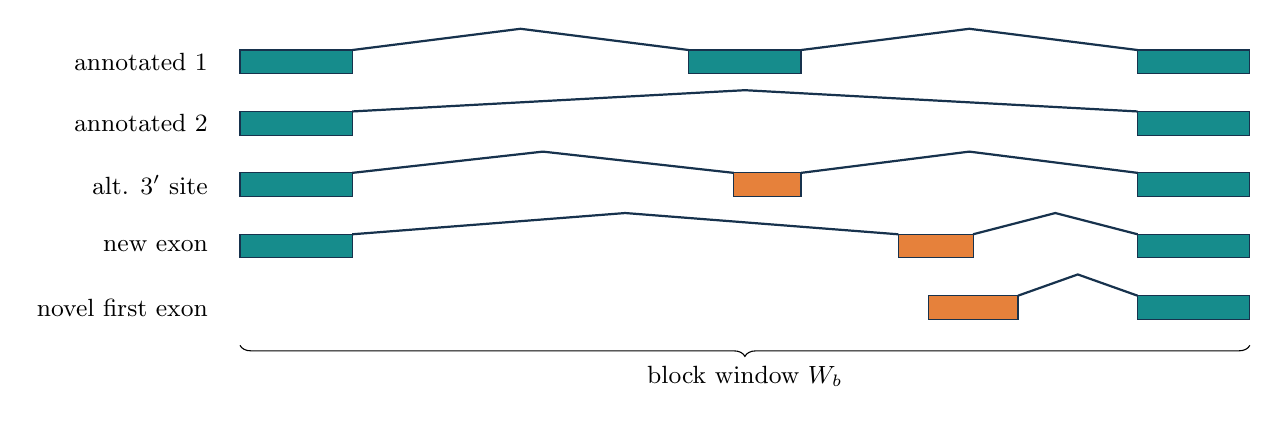
\begin{tikzpicture}[x=0.95mm,y=6mm,
  exon/.style={fill=tealeafTeal,draw=tealeafNavy},
  novel/.style={fill=tealeafOrange,draw=tealeafNavy},
  junction/.style={draw=tealeafNavy,thick}]
\def\pathlabel#1#2{\node[anchor=east,font=\small] at (-3,#1) {#2};}
% annotated paths
\pathlabel{0}{annotated 1}
\draw[exon] (0,-0.25) rectangle (15,0.25); \draw[exon] (60,-0.25) rectangle (75,0.25); \draw[exon] (120,-0.25) rectangle (135,0.25);
\draw[junction] (15,0.25) -- (37.5,0.7) -- (60,0.25); \draw[junction] (75,0.25) -- (97.5,0.7) -- (120,0.25);
\pathlabel{-1.3}{annotated 2}
\draw[exon] (0,-1.55) rectangle (15,-1.05); \draw[exon] (120,-1.55) rectangle (135,-1.05);
\draw[junction] (15,-1.05) -- (67.5,-0.6) -- (120,-1.05);
% alternative acceptor
\pathlabel{-2.6}{alt. 3$'$ site}
\draw[exon] (0,-2.85) rectangle (15,-2.35); \draw[novel] (66,-2.85) rectangle (75,-2.35); \draw[exon] (120,-2.85) rectangle (135,-2.35);
\draw[junction] (15,-2.35) -- (40.5,-1.9) -- (66,-2.35); \draw[junction] (75,-2.35) -- (97.5,-1.9) -- (120,-2.35);
% new exon
\pathlabel{-3.9}{new exon}
\draw[exon] (0,-4.15) rectangle (15,-3.65); \draw[novel] (88,-4.15) rectangle (98,-3.65); \draw[exon] (120,-4.15) rectangle (135,-3.65);
\draw[junction] (15,-3.65) -- (51.5,-3.2) -- (88,-3.65); \draw[junction] (98,-3.65) -- (109,-3.2) -- (120,-3.65);
% novel first exon
\pathlabel{-5.2}{novel first exon}
\draw[novel] (92,-5.45) rectangle (104,-4.95); \draw[exon] (120,-5.45) rectangle (135,-4.95);
\draw[junction] (104,-4.95) -- (112,-4.5) -- (120,-4.95);
% window
\draw[decorate,decoration={brace,mirror,amplitude=4pt}] (0,-6) -- (135,-6) node[midway,below=4pt,font=\small] {block window $W_b$};
\end{tikzpicture}
\caption{Novel paths in a block with two annotated paths (teal). Orange exons are created from novel junctions, an alternative acceptor in an existing exon, a new exon from a pair of novel junctions, and a novel first exon of length $T$ from a donor deep in an intron (more than 300 bases from any exon) whose junction pairs with no other.}
\label{fig:novel}
\end{figure}

\paragraph{New blocks.} Novel junctions inside a gene that lie in no annotated block window, for example a junction that skips an exon constitutive in the annotation, define new blocks. Such a junction is used if it satisfies the support criteria above, with $R^\star$ the largest read count of the annotated junctions overlapping it. Used junctions with overlapping introns are clustered. For a cluster with first donor $d$ and last acceptor $a$, each annotated transcript gives the segment of its exon chain from the exon to which $d$ attaches to the exon to which $a$ attaches; if only one end attaches, the segment starts at the last exon ending before $d$ or ends at the first exon starting after $a$, which allows novel first and last exons. Segments are clipped to their shared extent, distinct clipped segments are the annotated paths of the new block, and Algorithm~\ref{alg:novel} adds its novel paths. A new block is kept if it has at least one novel path.

\paragraph{Block set.} On the second pass the block set has 34{,}677 blocks, 22{,}898 annotated and 11{,}779 new, with 21{,}509 novel paths.

\section{Molecule classes}
\label{sec:classes}

\paragraph{Read compatibility.} For a read with aligned blocks $\{[\alpha_r,\beta_r)\}$ and junctions $\mathcal J_{\rm read}$, and a block $b$ whose window it overlaps, the read's blocks are clipped to $W_b$ and its junctions restricted to those inside $W_b$. The read is compatible with path $s$ (or the precursor path) if every clipped block lies within one exon of $E_s$ and every junction inside the window belongs to $J_s$. The read's class in block $b$ is the mask of compatible paths. A read of class 0, compatible with no path (for example a read with an unannotated junction not represented by a novel path, or a block reaching into an intron), is left out of the block. A molecule's class is the bitwise AND of the classes of its remaining reads that overlap the window; a molecule whose reads are compatible with disjoint sets of paths has class 0 and is discarded. A read enters every block of its locus whose window it overlaps.

\paragraph{Junction-only classes.} A junction is \emph{variable} in block $b$ if it belongs to some but not all mature paths. The junction-only collection keeps a molecule only if at least one of its reads of non-zero class has a variable junction inside the window.

\paragraph{Counts.} For each block, molecule counts are summed over the half-cell barcodes of each (subject, cell type, primer) and over sublibraries, giving $y_{ucpk}\in\mathbb N_0$ for subject $u$, cell type $c$, primer $p$ and class $k$. Internal blocks use the all-read counts and terminal blocks the junction-only counts.

\section{Read opportunities}

The probability of each class given the path composition is determined by read geometry. For path $s$ with spliced length $\lambda_s=\sum_i(y_{si}-x_{si})$, consider a read of length $L=151$ starting at every position $t\in\{1-L,\ldots,\lambda_s-1\}$ of the path's spliced sequence, so that it overlaps the path by at least one base, with the part outside the path clipped, as reads leaving the window are clipped in the data. The read's spliced interval is mapped to genomic blocks and junctions and classified with the same compatibility rule. The opportunity $n_{ks}\in\mathbb N_0$ is the number of start positions on path $s$ that give class $k$, and $L_s=\sum_kn_{ks}$ is the effective length of path $s$. For junction-only classes, only start positions whose read spans a variable junction count. Opportunities are computed for the $S_b$ mature paths and the precursor path.

Under a model in which molecules of path $s$ arise in proportion to an abundance $\rho_s$ per position and start uniformly along it, $P(\text{class }k)=\sum_s\rho_sn_{ks}/\sum_s\rho_sL_s$. The molecule share of path $s$ is $\pi_s=\rho_sL_s/\sum_{s'}\rho_{s'}L_{s'}$.

\section{Block test}
\label{sec:block}

\subsection{Projection and screens}

A test is indexed by a block $b$ and an unordered pair of cell types $\{c_0,c_1\}$, with $c_0$ the first in alphabetical order; effects are reported as $c_1$ minus $c_0$. The data of a test are the counts $y_{ucpk}$ for $c\in\{c_0,c_1\}$.
\begin{enumerate}[leftmargin=*]
  \item \textbf{Eligibility.} At least 4 subjects have molecules in both cell types, and the block has at least 20 molecules in the two cell types.
  \item \textbf{Same-junction groups (terminal blocks).} Paths with identical junction sets cannot be separated by junction-spanning reads and are merged into one group. A class is compatible with a group if it is compatible with any member, and the group opportunity is the mean of its members' opportunities. A block with fewer than two groups is not tested.
  \item \textbf{Share screen.} Molecule shares $\widehat{\bm\pi}$ are estimated from the class counts pooled over both cell types, both primers and all subjects, by the EM algorithm for $P(k)=\sum_s\pi_sn_{ks}/L_s$, with a pseudocount of 0.5 molecules per path per iteration (tolerance $10^{-10}$, at most 1{,}000 iterations). For internal blocks the precursor path is a component of the EM and is removed afterwards, with the mature shares renormalized. Paths with $\widehat\pi_s<0.01$ are removed. A block with fewer than two remaining paths is not a hypothesis and leaves the family. The screen uses no cell-type labels within the pair.
  \item \textbf{Projection.} Masks are restricted to the retained mature paths and the precursor bit is dropped. Molecules compatible only with the precursor or only with removed paths are discarded; classes that become identical are merged, with opportunities summed. The eligibility criteria are then applied again to the projected counts.
\end{enumerate}
After projection let $S$ be the number of retained paths and $K$ the number of classes.

\subsection{Likelihood of one path against the rest}

For target path $s$, the other paths are collapsed into one component with weights \[w_j=\frac{\widehat\pi_j/L_j}{\sum_{j'\ne s}\widehat\pi_{j'}/L_{j'}},\qquad j\neq s,\] the per-position abundances implied by the pooled molecule shares, so that the collapsed component's molecules divide among its paths in proportion to $\widehat\pi_j$. For class $k$ let \[\beta_k=n_{ks},\qquad \eta_k=\sum_{j\ne s}w_jn_{kj},\qquad B=\sum_k\beta_k,\qquad H=\sum_k\eta_k.\] All classes are kept, including the class compatible with all paths, whose relative frequency informs $\psi$ through coverage. For a subject--cell-type row $(u,c)$ with target usage $\psi\in(0,1)$, the class probabilities in primer $p$ are \[f_{pk}(\psi)=\frac{\psi_p\beta_k+(1-\psi_p)\eta_k}{\psi_pB+(1-\psi_p)H},\qquad \psi_p=\expit(\logit\psi+\gamma_p),\] with $\gamma_{\rm dT}=0$ and $\gamma_{\rm hex}=\gamma$, a primer offset that absorbs differences in positional capture between the primers. $\psi$ is the target's share of per-position abundance (the $\rho$ scale of the previous section), so its expected molecule share in primer $p$ is $\psi_pB/\{\psi_pB+(1-\psi_p)H\}$. Conditioning on the primer totals, the row log-likelihood is \[\ell_{uc}(\psi)=\sum_{p\in\{\mathrm{dT},\mathrm{hex}\}}\sum_{k=1}^Ky_{ucpk}\log f_{pk}(\psi).\] 
\paragraph{Primer offset.} $\gamma$ is estimated before the test without cell-type labels, by maximizing the profile likelihood in which every row has its own usage, \[\widehat\gamma=\arg\max_{\gamma\in[-4,4]}\sum_{(u,c)}\max_{t\in\mathbb R}\left[\ell_{uc,\mathrm{dT}}(\expit t)+\ell_{uc,\mathrm{hex}}(\expit(t+\gamma))\right],\] over rows observed with both primers, where $\ell_{uc,p}$ is the primer-$p$ term of $\ell_{uc}$. The maximization uses a grid of step 0.05 in $\gamma$ and in $t\in[-22,22]$, refined by a parabola through the three best points. $\widehat\gamma$ is estimated for each target path and held fixed in both hypotheses.

\subsection{Random-effects model}

Let $z_c=\mathbf 1[c=c_1]$. Usage varies between subjects through a subject intercept and between rows through a Beta distribution, \[v_u\sim\mathcal N(0,\sigma^2),\qquad \mu_{uc}=\expit(\theta_0+\theta_1z_c+v_u),\qquad \psi_{uc}\mid v_u\sim\BetaDist\big(\kappa\mu_{uc},\kappa(1-\mu_{uc})\big),\] with fixed effects $\theta_0,\theta_1\in\mathbb R$, subject standard deviation $\sigma>0$ and row concentration $\kappa>0$. The subject intercept is shared by the subject's two cell types, which makes the test paired. Subjects observed in only one cell type contribute to $\theta_0$, $\sigma$ and $\kappa$. The marginal likelihood is \[\mathcal L(\theta_0,\theta_1,\kappa,\sigma)=\prod_u\int_{\mathbb R}\phi(v;0,\sigma^2)\prod_{c\in\mathcal C_u}\int_0^1e^{\ell_{uc}(\psi)}\,\BetaDist\big(\psi;\kappa\mu_{uc}(v),\kappa(1-\mu_{uc}(v))\big)\,d\psi\,dv,\] where $\mathcal C_u$ is the set of cell types observed for subject $u$.

\paragraph{Numerical integration.} The inner integral is evaluated in $t=\logit\psi$ on $[-18,18]$ by the trapezoid rule, with the tails beyond $\pm18$ added analytically at the boundary value of $\ell_{uc}$. The grid spacing for row $(u,c)$ is $\min\{0.03,\,s_{uc}/1.5\}$, where $s_{uc}$ is a quarter of the width of the region where $\ell_{uc}(\expit t)$ is within 2 of its maximum. The outer integral uses adaptive Gauss--Hermite quadrature with 9 nodes, centred on each subject's posterior mode $\widehat v_u$ (damped Newton iterations) and scaled by the inverse square root of the negative second derivative of the log integrand at the mode.

\paragraph{Estimation.} Maximum-likelihood estimates are found by the L-BFGS-B algorithm with analytic gradients in the coordinates $(\theta_0,\theta_1,\log\kappa,\log\sigma)$, within the bounds $-12\le\theta_0,\theta_1\le12$, $0.1\le\kappa\le2000$ and $0.01\le\sigma\le3$. The null fit ($\theta_1=0$) starts from least-squares coefficients on the rows' maximum-likelihood usages, $\kappa=20$ and $\sigma=0.5$; the alternative starts from the null solution, and is refitted from $\theta_1=0$ if it ends below the null log-likelihood.

\paragraph{Test.} With $(\widehat\theta_0,\widehat\theta_1,\widehat\kappa,\widehat\sigma)$ the alternative and $(\widetilde\theta_0,0,\widetilde\kappa,\widetilde\sigma)$ the null estimates, the statistic is \[T_s=2\left\{\log\mathcal L(\widehat\theta_0,\widehat\theta_1,\widehat\kappa,\widehat\sigma)-\log\mathcal L(\widetilde\theta_0,0,\widetilde\kappa,\widetilde\sigma)\right\},\] and $p_s=P(\chi^2_1>T_s)$. Both optima are re-evaluated at half the $\psi$ grid spacing and 19 quadrature nodes; if the log-likelihoods or the statistic change by more than $10^{-3}$, the test is refitted at the finer setting and checked again at quarter spacing and 39 nodes. A test is converged if both fits succeed and the change is at most $10^{-3}$; the reported statistic is $\max(T_s,0)$ at the finer setting. A path test that does not converge has $p_s=1$.

\subsection{Block p-value and effect}

For $S=2$ there is one test, of path 1. For $S>2$, each of the $S$ paths is tested against the rest and the block p-value is the Simes combination \[p_b=\min\left\{1,\ \min_{i=1,\ldots,S}\frac{S\,p_{(i)}}{i}\right\},\] where $p_{(1)}\le\cdots\le p_{(S)}$ are the ordered path p-values. The effect for $S=2$ is $\bar m_{c_1}-\bar m_{c_0}$ for path 1 (and its negative for path 2), where $\bar m_c=\int\expit(\widehat\theta_0+\widehat\theta_1z_c+v)\phi(v;0,\widehat\sigma^2)\,dv$ is the marginal usage on the poly(dT) scale. For $S>2$, the molecule-share composition of each row is estimated by the EM algorithm of the share screen with primers pooled, compositions are averaged over the subjects observed in both cell types, and the effect is the difference of the averages.

\subsection{Hypothesis family}

Internal-block tests and terminal-block tests form one family, with BH applied over all tests of a cohort. A test that fails to converge, or has fewer than four subjects in its fit, enters with $p=1$; a block removed by a screen does not enter.

\section{Calibration}

Calibration is checked by count simulations under the null on real designs. For randomly chosen blocks and cell-type pairs of the full data (200 for internal and 800 for terminal blocks, on the 1{,}163-gene block set of an earlier target list), the observed molecule totals per (subject, cell type, primer) are kept, and class counts are redrawn from compositions in which the two cell types share the same path usage. A subject composition is drawn from a Dirichlet distribution with concentration 20 around the pooled shares, the row composition from a Dirichlet with concentration $\varsigma\in\{5,20,\infty\}$ around the subject composition, and class counts from the multinomial implied by the opportunities, two draws per test. Internal tests reject at most 2.9\% of converged fits at nominal 0.05 and at most 1.0\% at 0.01. Junction-only terminal tests reject 3.4--4.3\% (two-path) and 2.7--4.1\% (multi-path) at 0.05, at most 1.1\% at 0.01 and at most 0.5\% at 0.001.

\section{Evaluation}
\label{sec:evaluation}

\subsection{Subject-split replication}

The 48 subjects are divided into two halves of 24 with 4 subjects of each group in each half (subjects shuffled within group and assigned alternately). Tealeaf and every comparator are fitted separately on each half. For each comparator $m$, the universe $\mathcal K_m$ is the set of (gene, cell-type pair) keys with a finite p-value for $m$ in both halves, taken from the comparator's own results, over up to 190 cell-type pairs; no Tealeaf result enters it. SUPPA2 and primer-aware SUPPA2 use exact paired signed-rank tests over the full event catalogue. An earlier SUPPA2/Tealeaf hybrid comparator, SUPPA2 events quantified with an earlier Tealeaf transcript model, is not used: its directions agree with the long reads at chance ($A_{100}=0.567$, 49 of its 100 top-ranked events agree), so its replicated genes do not reflect splicing differences confirmed by an independent measurement. Tealeaf is fitted on every key of these universes. Each comparison is scored on two universes, the \emph{matched} universe $\mathcal U_m=\mathcal K_m\cap\mathcal T_1\cap\mathcal T_2$, with $\mathcal T_h$ the keys with a Tealeaf test in half $h$, and the \emph{comparator} universe $\mathcal K_m$. In each half $h$, block p-values of a (gene, pair) key are combined by Simes, keys of the universe without a test receive $p=1$, and the key p-values of a gene are combined by Simes into $p_{gh}$. Comparator feature p-values (LeafCutter intron clusters, MAJIQ Heterogen edges, scQuint intron groups, SUPPA2 and rMATS events) are aggregated in the same way. The conjunction p-value $p_g^{\rm rep}=\max(p_{g1},p_{g2})$ tests for signal in both halves, and a gene is \emph{replicated} if its BH-adjusted conjunction p-value over the genes of the universe is at most 0.05; both methods are scored on the same universe. Replication does not require agreement of direction.

\subsection{Long-read direction}

Directions of full-data tests are compared with the P56 mouse brain single-cell long-read data of Joglekar et al.\ (ScISOr-Seq2), using its UMI-filtered annotated-transcript count matrix. Transcript names are matched to the comprehensive GENCODE vM32 annotation, which gives each counted transcript an exon chain. Eight cell types have a prespecified correspondence, astrocytes (with Bergmann glia), mature oligodendrocytes, cerebellar granule neurons, cortical excitatory neurons, dentate gyrus and CA excitatory neurons, thalamic excitatory neurons and medium spiny neurons; glial samples are pooled over regions within replicate. The full data are tested on all pairs of these eight cell types in addition to the split universe. A transcript counts for a tested path if its exon chain is compatible with that path and no other, by the rule used for reads (Section~\ref{sec:classes}): its exons clipped to the block window lie within exons of the path and its junctions inside the window are junctions of the path. Transcripts compatible with several paths, which do not cover the region where the paths differ, and transcripts compatible with none are not counted. A novel path is evaluable when an annotated transcript of the comprehensive annotation has its structure. A test is evaluable if every tested path has at least one counted transcript, both cell types have at least 20 counted long-read UMIs, and both effects are finite and non-zero; 34{,}634 tests are evaluable. With long-read counts $\bm n_c\in\mathbb N_0^S$ of the paths in cell type $c$ (summed over replicates and over the transcripts of each path), the long-read effect is $\bm\Delta^{\rm L}=\bm n_{c_1}/\|\bm n_{c_1}\|_1-\bm n_{c_0}/\|\bm n_{c_0}\|_1$, and the test agrees if $(\bm\Delta^{\rm T})^{\mathsf T}\bm\Delta^{\rm L}>0$ for the Tealeaf effect $\bm\Delta^{\rm T}$. Evaluable tests are ranked by p-value, then by decreasing statistic. With $a_j\in\{0,1\}$ the agreement of the test at rank $j$ and $c_r=r^{-1}\sum_{j\le r}a_j$ the cumulative agreement, the endpoint is the normalized area $A_{100}=\frac{1}{100}\sum_{r=1}^{100}c_r$, the mean cumulative agreement over the 100 top-ranked tests. Comparators are ranked and scored in the same way, with long-read counts assigned by the same annotation and the same use of exon chains: junction usage of LeafCutter, MAJIQ and scQuint features is computed from the junctions of each counted transcript's exon chain on both strands, and each event of SUPPA2 and rMATS is scored from transcripts whose exon chain has its inclusion or its exclusion form.

\subsection{Results of the current model}

\begin{table}[ht]
\centering
\small
\setlength{\tabcolsep}{4pt}
\begin{tabular}{lcccccc}
\toprule
 & LeafCutter & MAJIQ & SUPPA2 & SUPPA2-PA & rMATS & scQuint\\
\midrule
\multicolumn{7}{l}{\emph{Matched universe}}\\
Genes & 263 & 2{,}764 & 3{,}411 & 3{,}072 & 5{,}070 & 3{,}603\\
Tealeaf replicated & 64 & 201 & 124 & 130 & 158 & 179\\
Comparator replicated & 35 & 27 & 8 & 0 & 4 & 135\\
\midrule
\multicolumn{7}{l}{\emph{Comparator universe}}\\
Genes & 279 & 3{,}003 & 5{,}068 & 3{,}901 & 6{,}838 & 4{,}220\\
Tealeaf replicated & 64 & 196 & 101 & 115 & 136 & 172\\
Comparator replicated & 36 & 28 & 0 & 0 & 4 & 124\\
\midrule
Comparator $A_{100}$ & .918 & .938 & .870 & .625 & .898 & .914\\
\bottomrule
\end{tabular}
\caption{Replicated genes on each comparator's matched and comparator universes, and long-read direction. SUPPA2-PA is primer-aware SUPPA2. Tealeaf has $A_{100}=0.940$ (93 of its 100 top-ranked evaluable tests agree with long reads; $A_{40}=0.959$, $A_{200}=0.936$).}
\label{tab:results}
\end{table}

Table~\ref{tab:results} gives both endpoints. On both the matched and the comparator universes Tealeaf replicates more genes than every comparator. Figure~\ref{fig:lr} shows cumulative long-read agreement by rank. Over the first 40 ranks MAJIQ and scQuint agree slightly more often than Tealeaf; at rank 100 Tealeaf ($A_{100}=0.940$, 93 agreeing) is level with MAJIQ (0.938, 85 agreeing), and by rank 200 Tealeaf still agrees for 94\% of its tests against 75--84\% for the junction methods and 80\% for rMATS. Tealeaf has 34{,}634 evaluable tests against 1{,}562 to 8{,}497 features for the junction methods. The SUPPA2 and rMATS values are computed on their 500 top-ranked events per contrast.

\begin{figure}[ht]
\centering
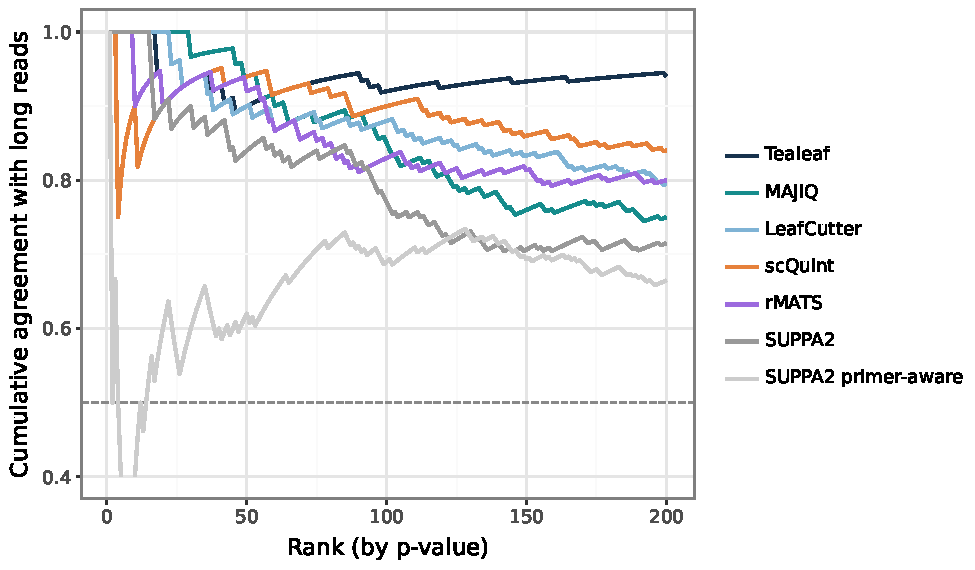
\includegraphics[width=0.85\textwidth]{figures/lr_agreement.pdf}
\caption{Cumulative agreement with long-read directions among the top-ranked tests (Tealeaf) or features (comparators), ranked by p-value; the dashed line is chance. Long-read counts are assigned by each transcript's exon chain in the comprehensive annotation for all methods.}
\label{fig:lr}
\end{figure}

\subsection{Event classes}

Each test is assigned an event class from the exon chains of its retained paths. If all chains start and end at the same bases the block is internal, and two chains are classified by the exons in which they differ as a cassette exon, multi-exon skipping, an alternative donor or acceptor, mutually exclusive exons or a retained intron (a differing pattern outside these is complex internal); more than two chains are compound internal. Otherwise the paths differ at a transcript end, an alternative first exon, an alternative last exon, or both, oriented by the strand; when the differing terminal exons share their splice site, only the transcript start or end moves. Table~\ref{tab:events} gives the full-data tests, BH discoveries at 0.05 (one family over internal and terminal blocks) and their long-read agreement by class. Most discoveries that retain a novel path have no long-read counterpart. Long-read agreement of discoveries is 0.79 to 0.91 for the common classes, highest for alternative first exons and cassette exons. Retained introns are rare among block tests because a path whose chain is the whole window is removed; a per-intron test of differential retention is described in Appendix~\ref{sec:ir}.

\begin{table}[ht]
\centering
\footnotesize
\setlength{\tabcolsep}{4pt}
\begin{tabular}{lrrrrr}
\toprule
Event class & Tests & Discoveries & Novel path & LR agreement & Top 100\\
\midrule
cassette exon & 215{,}456 & 3{,}549 & 1{,}551 & 0.88 (449) & 38/39\\
alternative first exon & 104{,}601 & 2{,}837 & 2{,}115 & 0.91 (139) & 22/23\\
compound internal & 101{,}871 & 1{,}614 & 1{,}208 & 0.84 (77) & 3/3\\
alternative last exon & 69{,}974 & 1{,}060 & 628 & 0.86 (85) & 21/25\\
alternative first and last exons & 24{,}167 & 851 & 689 & 0.79 (39) & 2/3\\
alternative acceptor & 99{,}219 & 313 & 249 & 0.83 (41) & 3/3\\
alternative donor & 55{,}749 & 113 & 89 & 0.53 (15) & 1/1\\
alternative transcript end & 4{,}415 & 100 & 13 & 1.00 (7) & 0/0\\
multi-exon skipping & 8{,}885 & 99 & 57 & 0.90 (21) & 3/3\\
mutually exclusive exons & 2{,}701 & 82 & 11 & 0.88 (8) & 0/0\\
complex internal & 4{,}867 & 59 & 57 & 1.00 (3) & 0/0\\
alternative transcript start & 2{,}113 & 52 & 1 & 1.00 (3) & 0/0\\
retained intron & 935 & 13 & 13 & -- (0) & 0/0\\
\bottomrule
\end{tabular}
\caption{Full-data tests by event class. Novel path counts discoveries that retain an unannotated path. LR agreement is the fraction of long-read-evaluable discoveries whose direction agrees with the long reads (number evaluable in parentheses); Top 100 gives agreeing over all tests of the class among the 100 top-ranked long-read-evaluable tests.}
\label{tab:events}
\end{table}

Figure~\ref{fig:discoveries} compares full-data discoveries with the comparators on the 28 pairs of the eight long-read cell types, the contrasts every method tests on the full data. Each method's finite p-values on these contrasts form one BH family, and a discovery has adjusted p at most 0.05. Methods test different units, a block for Tealeaf, an intron cluster for LeafCutter, an intron group for scQuint, a local splice variant for MAJIQ and an event for SUPPA2 and rMATS, so discoveries are also counted as gene--cell-type pairs with at least one discovery. Tealeaf has 3{,}631 discoveries in 3{,}020 gene--cell-type pairs, scQuint 2{,}234 pairs, MAJIQ 873, LeafCutter 351, SUPPA2 350, primer-aware SUPPA2 233 and rMATS 164. SUPPA2 and rMATS events are mapped to the Tealeaf classes (skipped exon to cassette exon, alternative 5$'$ and 3$'$ splice sites to alternative donor and acceptor, and mutually exclusive exons and retained introns to themselves); their event sets contain no alternative first or last exons, which make up 1{,}508 of the Tealeaf discoveries. Tealeaf discovers 1{,}024 cassette exons against 321 for SUPPA2 and 166 for rMATS. Over all 190 cell-type pairs (Figure~\ref{fig:discoveries-all}), with LeafCutter tested on 171, MAJIQ on 170 and SUPPA2 on 135 of them, Tealeaf has 10{,}742 discoveries in 9{,}037 gene--cell-type pairs, scQuint 8{,}835 pairs, MAJIQ 2{,}189, LeafCutter 890, rMATS 570, primer-aware SUPPA2 533 and SUPPA2 280. Tealeaf discovers 3{,}549 cassette exons against 495 for rMATS and 493 for primer-aware SUPPA2.

\begin{figure}[ht]
\centering
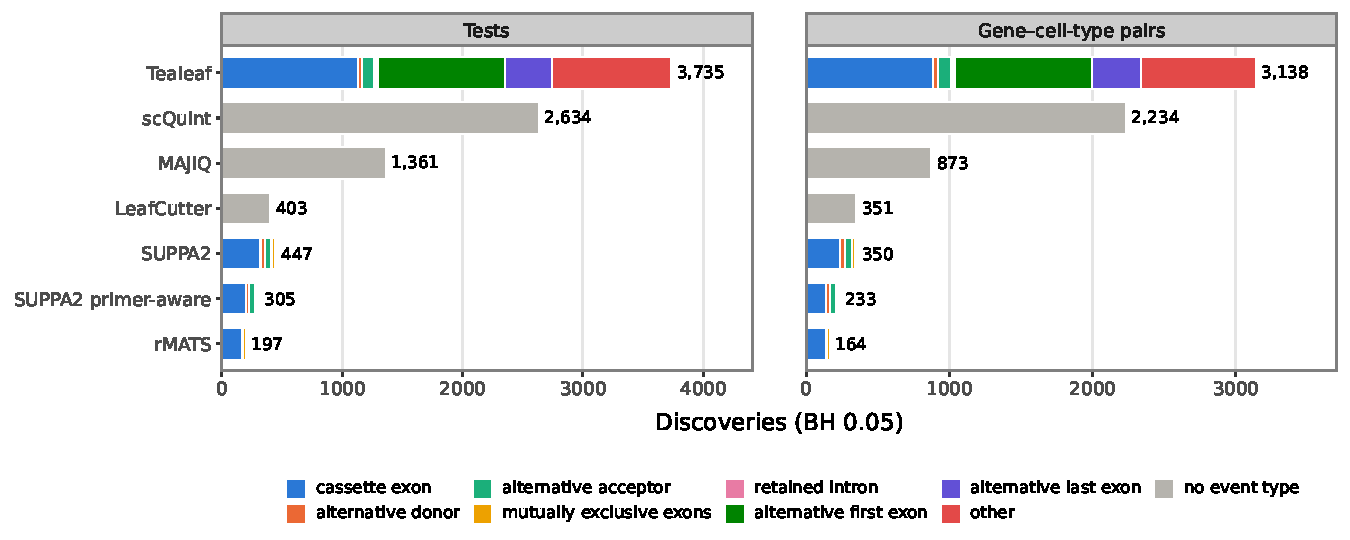
\includegraphics[width=\textwidth]{figures/discoveries_by_event.pdf}
\caption{Full-data discoveries (BH 0.05 within method) on the 28 cell-type pairs tested by every method, counted as tests (left) and as gene--cell-type pairs with at least one discovery (right), by event class. A gene--cell-type pair takes the class of its smallest-p discovery. Other collects the Tealeaf classes without a comparator counterpart, compound and complex internal, multi-exon skipping, alternative first and last exons together, and alternative transcript start or end. LeafCutter, scQuint and MAJIQ test junction clusters, which have no event type.}
\label{fig:discoveries}
\end{figure}

\begin{figure}[ht]
\centering
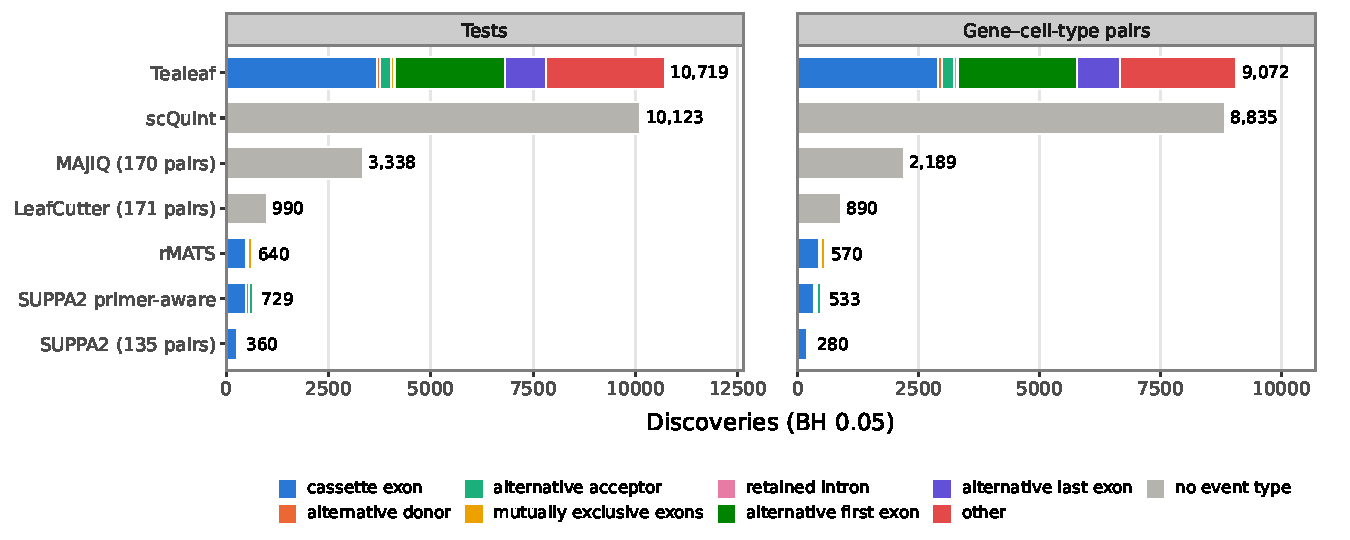
\includegraphics[width=\textwidth]{figures/discoveries_by_event_all.pdf}
\caption{Full-data discoveries as in Figure~\ref{fig:discoveries}, on all 190 cell-type pairs each method tests; methods tested on fewer pairs give their number of pairs.}
\label{fig:discoveries-all}
\end{figure}

\subsection{Examples}

Figures~\ref{fig:pkn2}--\ref{fig:mctp1} show the full-data tests with the largest effect among those evaluable in the long-read data, selected without regard to long-read agreement: tests with $p<10^{-8}$, at least 50 long-read UMIs per cell type and at most four paths, one per gene, ranked by the norm of the fitted path-usage difference, with at least one internal and one terminal block. Each figure shows sashimi plots of Parse coverage by primer and of the coverage implied by the long-read transcript counts, over the whole gene with all its annotated transcripts and zoomed in on the block with its paths, and Figure~\ref{fig:usage} shows the molecule-share composition of every subject--cell-type row in the Parse data (the per-row EM estimate of the share screen) and the transcript share of each path in the two long-read replicates. All four agree with the long reads in direction.
\begin{enumerate}[leftmargin=*]
  \item \textbf{Pkn2} (Figure~\ref{fig:pkn2}), a cassette exon. Path 2 includes the exon. Astrocytes include it in 68\% of molecules and cortical excitatory neurons in 27\% (means over 13 subjects with both cell types); the long reads show inclusion in 100\% and 87\% of the transcripts that span the block (229 and 276 UMIs). The direction agrees, but the levels differ in cortical neurons, which skip the exon in 73\% of Parse molecules and 13\% of long-read transcripts.
  \item \textbf{Nfasc} (Figure~\ref{fig:nfasc}), a short cassette exon included by path 2. Cortical excitatory neurons include it in 89\% of molecules and oligodendrocytes in 16\% (47 subjects). The long reads agree in direction (19\% and 1\% of transcripts) but put most cortical neuron transcripts on the skipping path.
  \item \textbf{Kif21a} (Figure~\ref{fig:kif21a}), a 21-base cassette exon included by path 3. The block has a second 21-base exon (path 2), which carries 0.4\% of molecules and is removed by the share screen, so the test compares paths 1 and 3. Path 3 is used in 71\% of cortical neuron and 41\% of oligodendrocyte molecules (29 subjects); the long-read shares are 72\% and 46\%.
  \item \textbf{Mctp1} (Figure~\ref{fig:mctp1}), an alternative first exon in a terminal block, with the two first exons tens of kilobases apart, so the sashimi view is dominated by intronic coverage and the exons are narrow; the junction arcs carry the comparison. Paths 2 and 3 share their junctions and differ only in where their first exon starts, so the junction-only test merges them. Dentate gyrus granule neurons use the upstream first exon (path 1) in 74\% of junction-spanning molecules and medium spiny neurons in 15\% (8 subjects); the long-read shares are 33\% and 18\%.
\end{enumerate}

\begin{figure}[p]
\centering
\makebox[\textwidth][c]{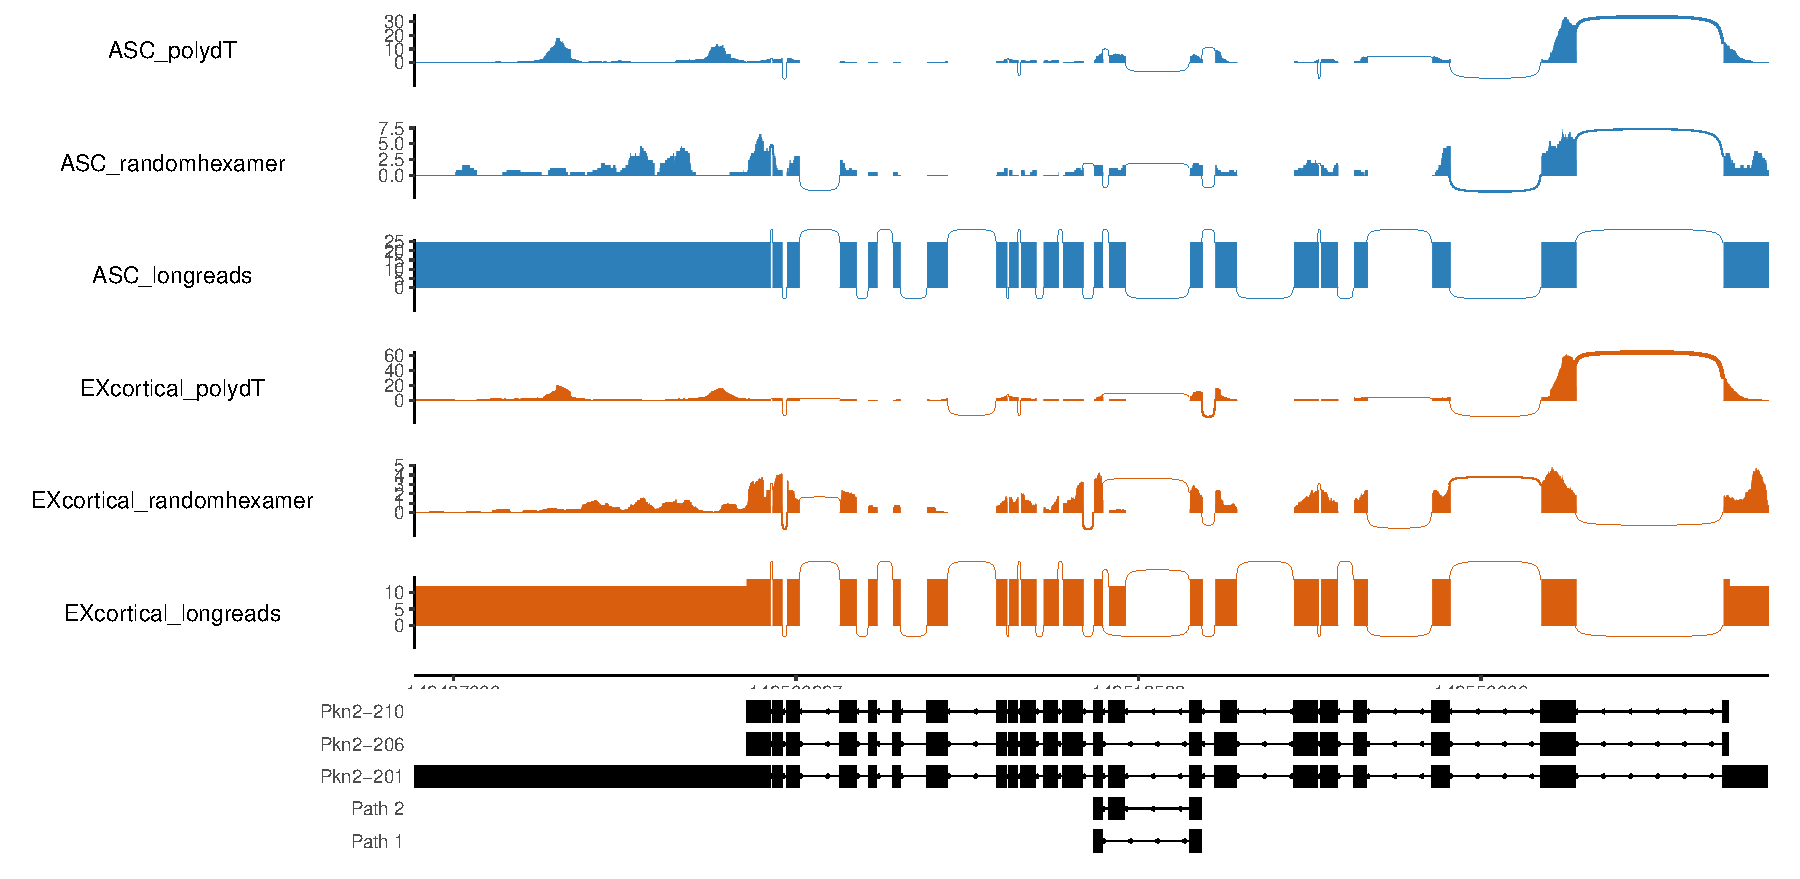
\includegraphics[width=1.15\textwidth,height=0.36\textheight,keepaspectratio]{figures/sashimi_Pkn2_B3_gene.pdf}}\\
(a)\\[4pt]
\makebox[\textwidth][c]{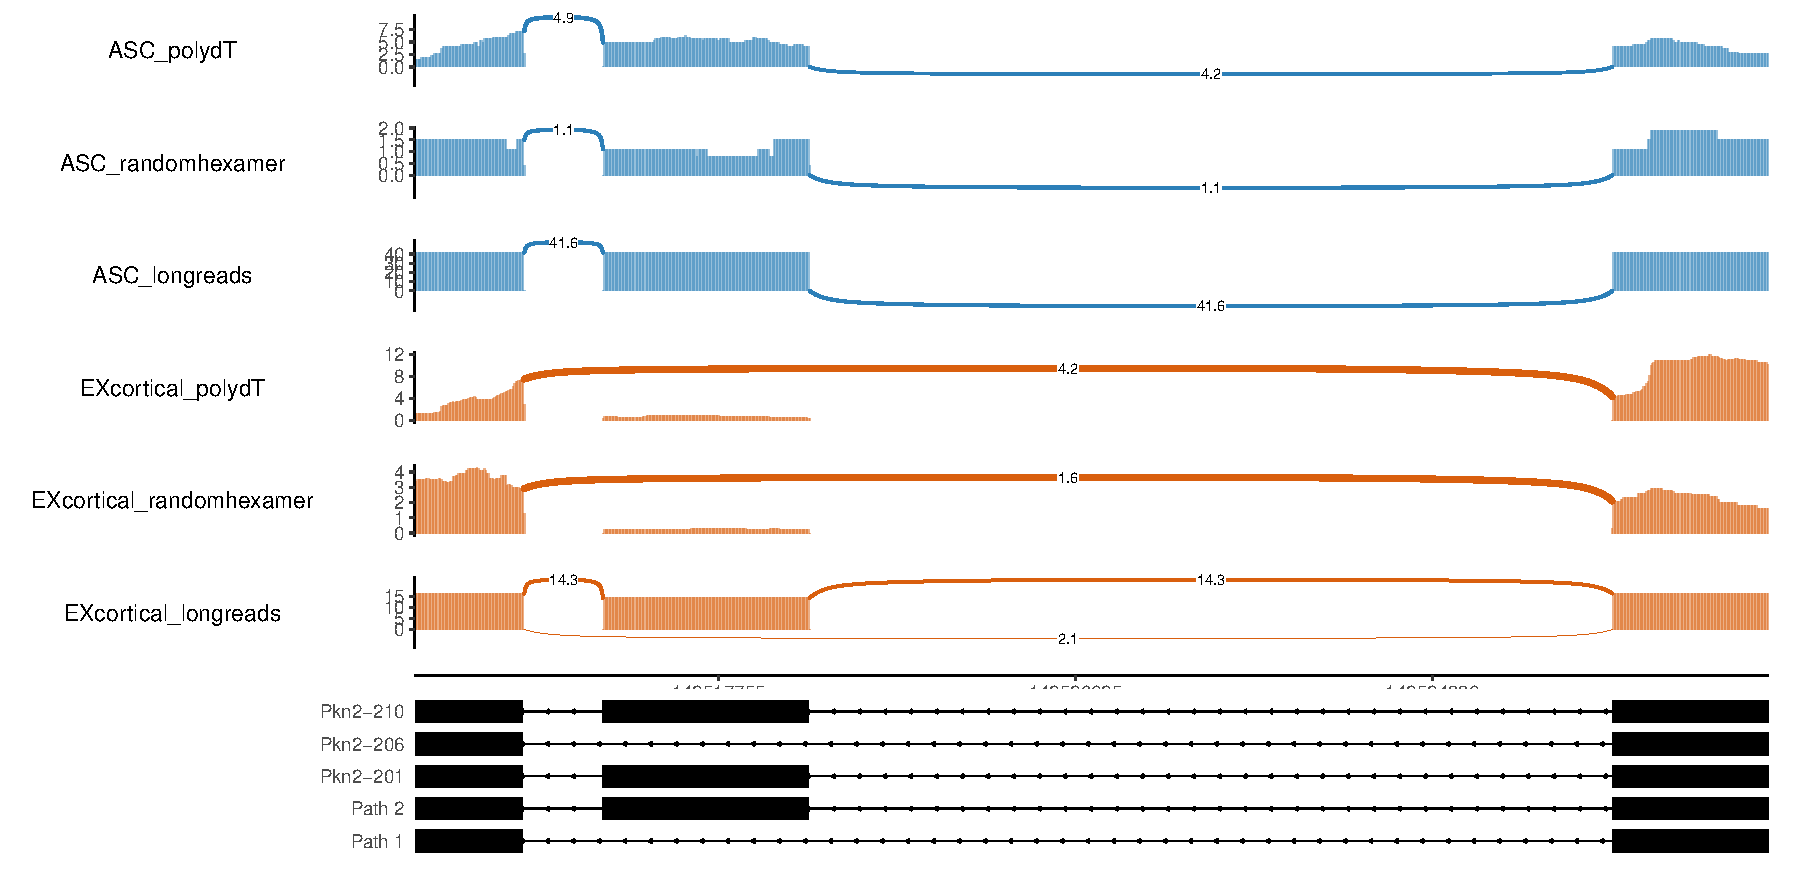
\includegraphics[width=1.15\textwidth,height=0.36\textheight,keepaspectratio]{figures/sashimi_Pkn2_B3.pdf}}\\
(b)
\caption{Pkn2 block 3, astrocytes against cortical excitatory neurons. (a) Sashimi tracks over the whole gene and (b) over the block, for the two cell types: Parse coverage from UMI-deduplicated native alignments by primer, per 1,000 half-cells of the primer, and long-read coverage implied by the UMI counts of full-length annotated transcripts (summed over the two replicates), per million long-read UMIs of the cell type. Arcs are junctions, labelled with their coverage in the same units in the block view, and long introns are shortened. Below the tracks are the block's paths (Path $k$), which mark the block in the gene view, and the gene's annotated transcripts.}
\label{fig:pkn2}
\end{figure}

\begin{figure}[p]
\centering
\makebox[\textwidth][c]{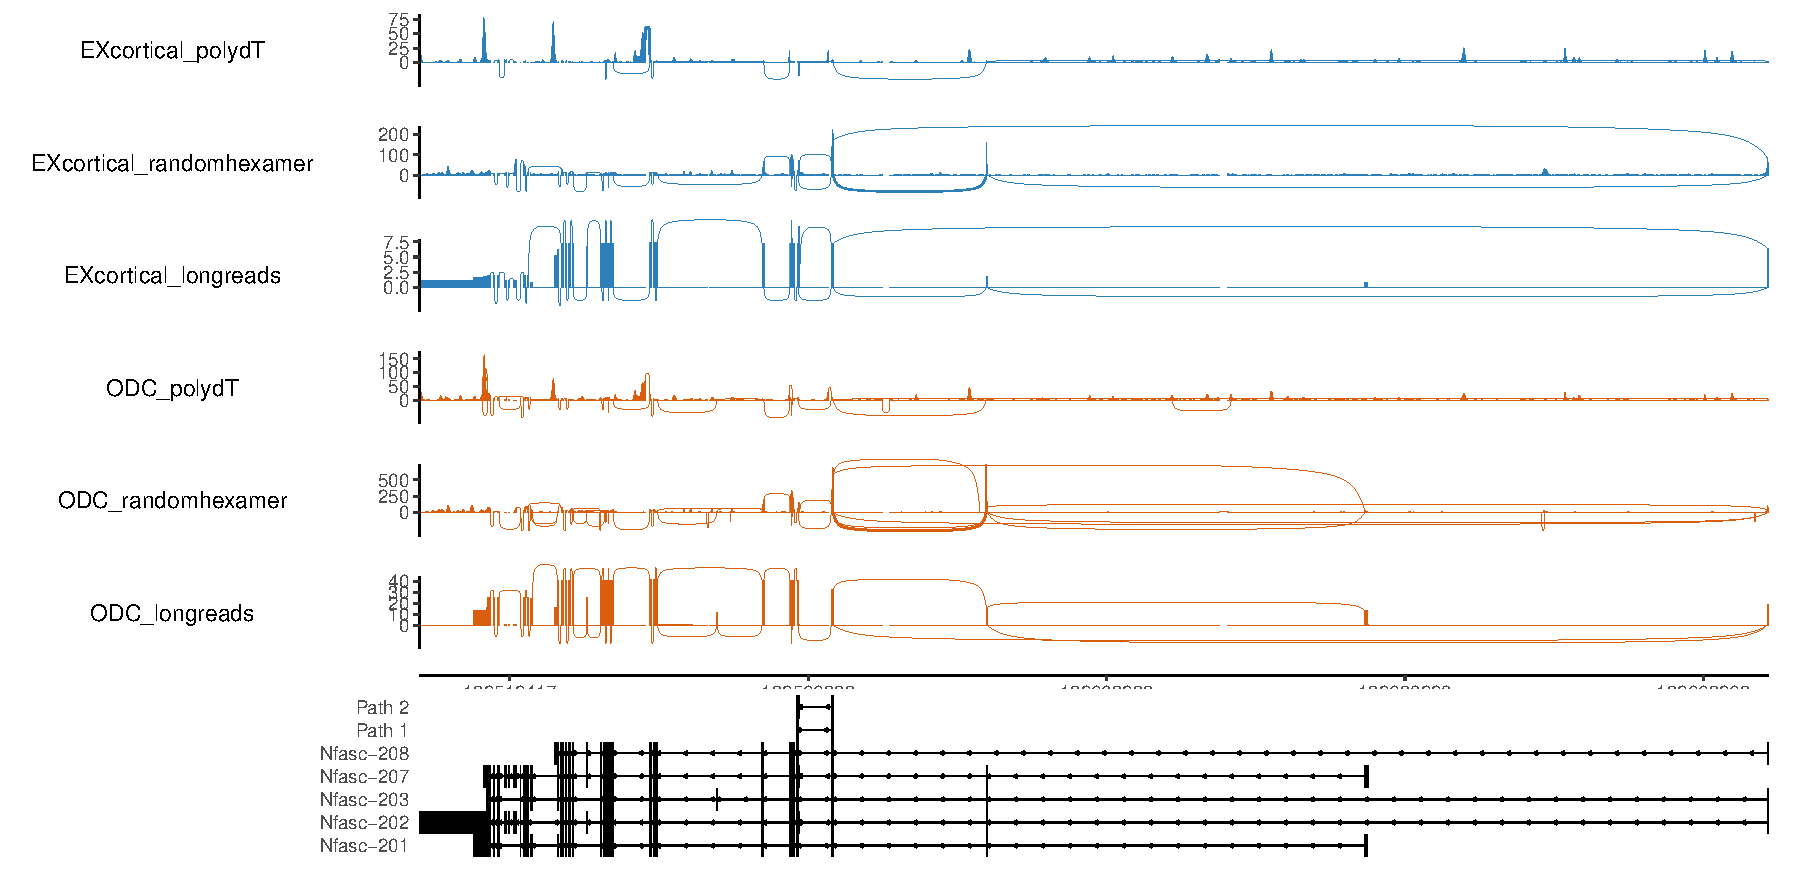
\includegraphics[width=1.15\textwidth,height=0.4\textheight,keepaspectratio]{figures/sashimi_Nfasc_B2_gene.pdf}}\\
(a)\\[4pt]
\makebox[\textwidth][c]{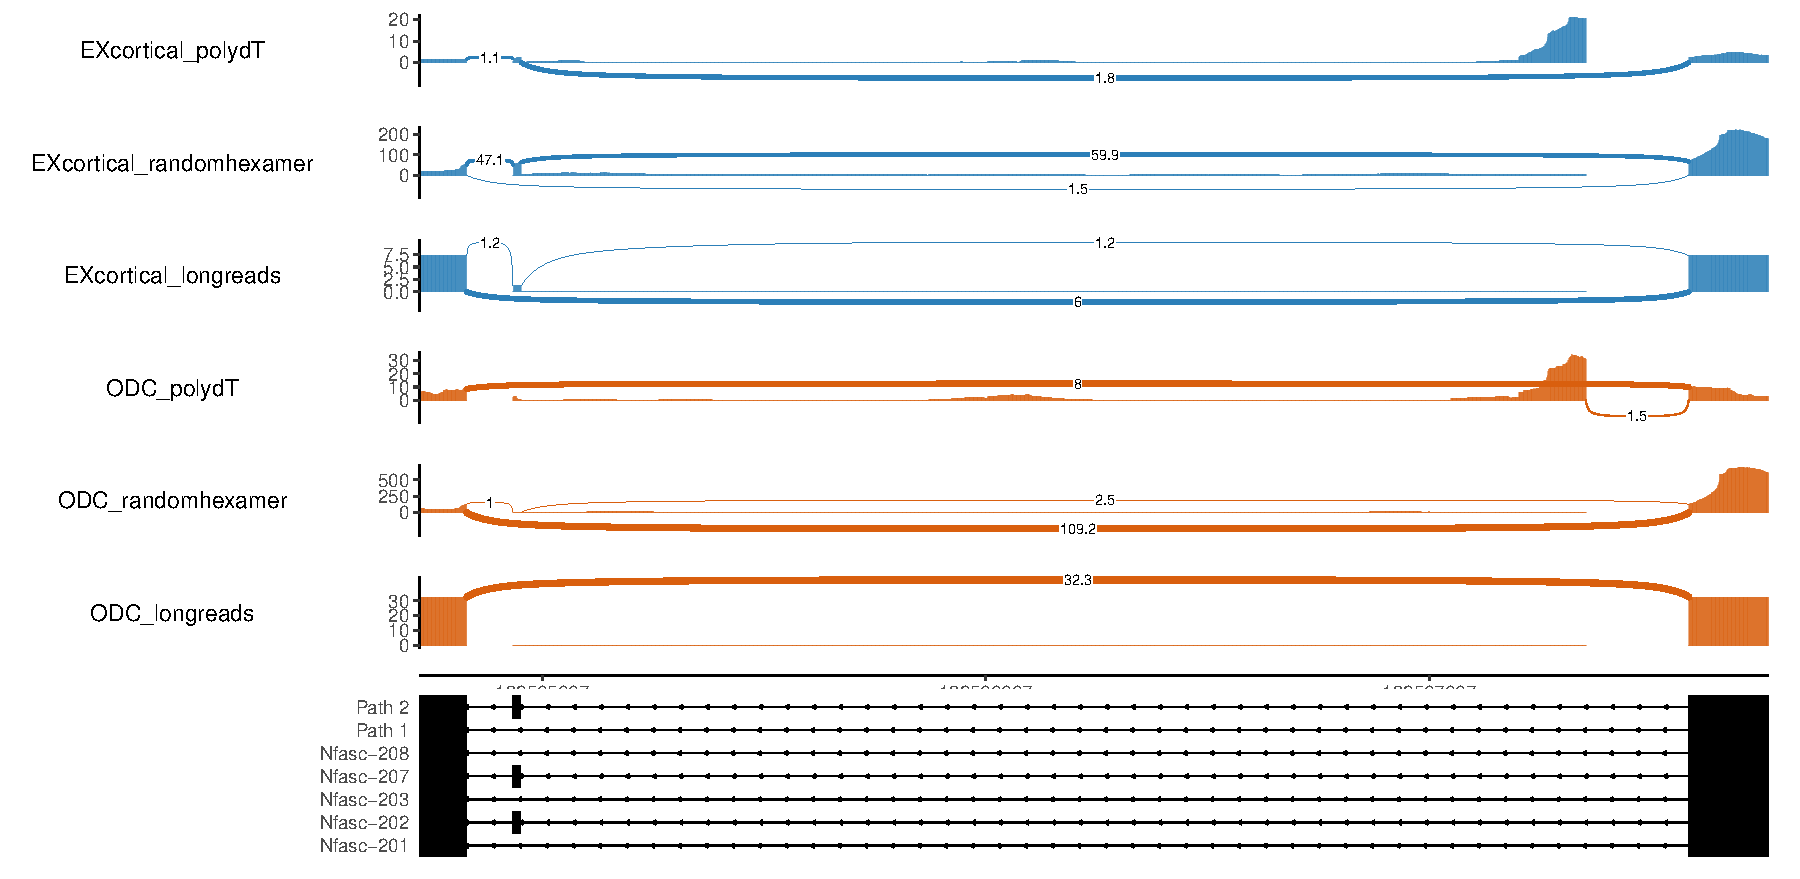
\includegraphics[width=1.15\textwidth,height=0.4\textheight,keepaspectratio]{figures/sashimi_Nfasc_B2.pdf}}\\
(b)
\caption{Nfasc block 2, cortical excitatory neurons against oligodendrocytes. Panels as in Figure~\ref{fig:pkn2}.}
\label{fig:nfasc}
\end{figure}

\begin{figure}[p]
\centering
\makebox[\textwidth][c]{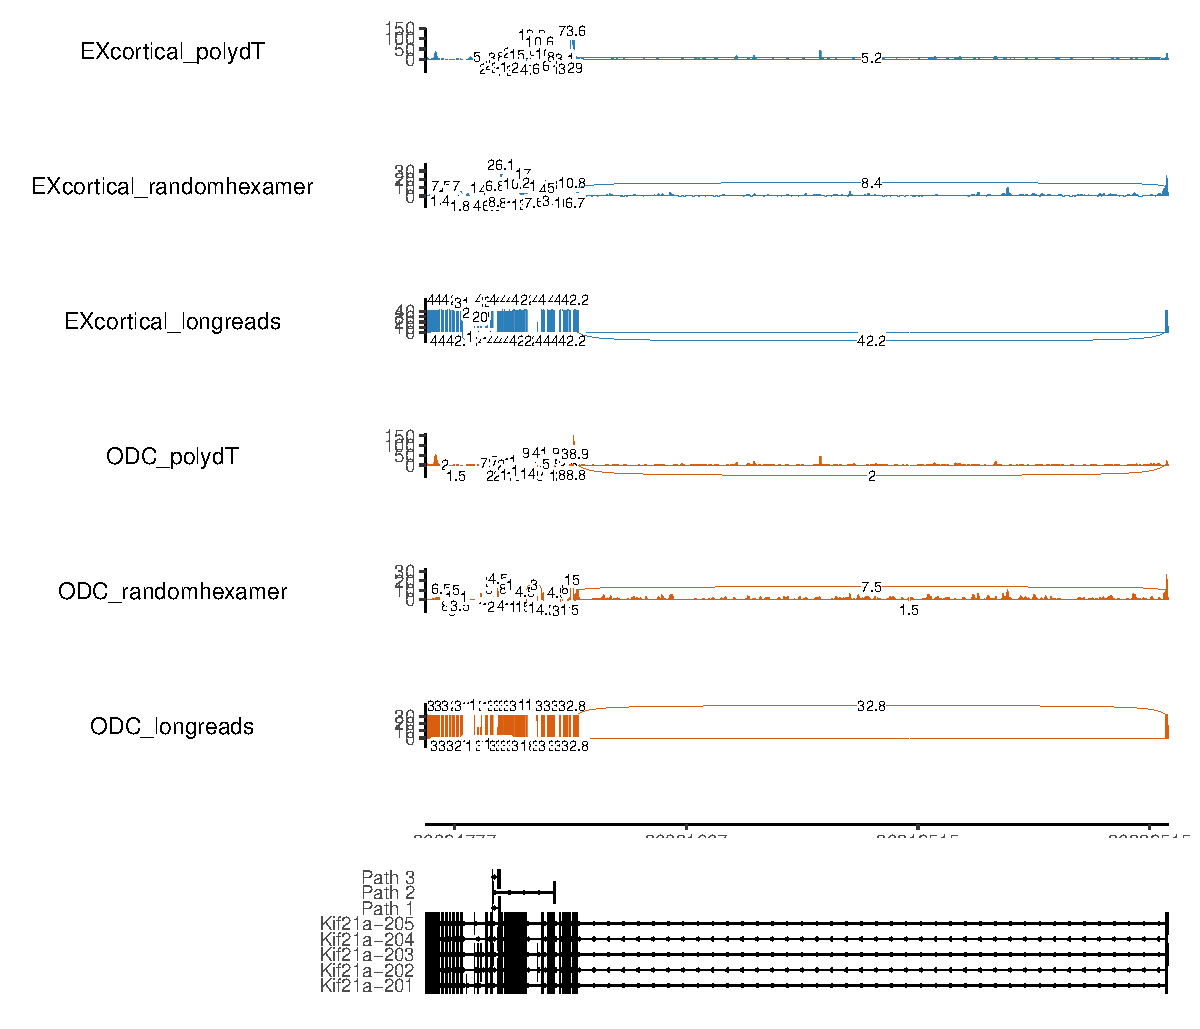
\includegraphics[width=1.15\textwidth,height=0.4\textheight,keepaspectratio]{figures/sashimi_Kif21a_B3_gene.pdf}}\\
(a)\\[4pt]
\makebox[\textwidth][c]{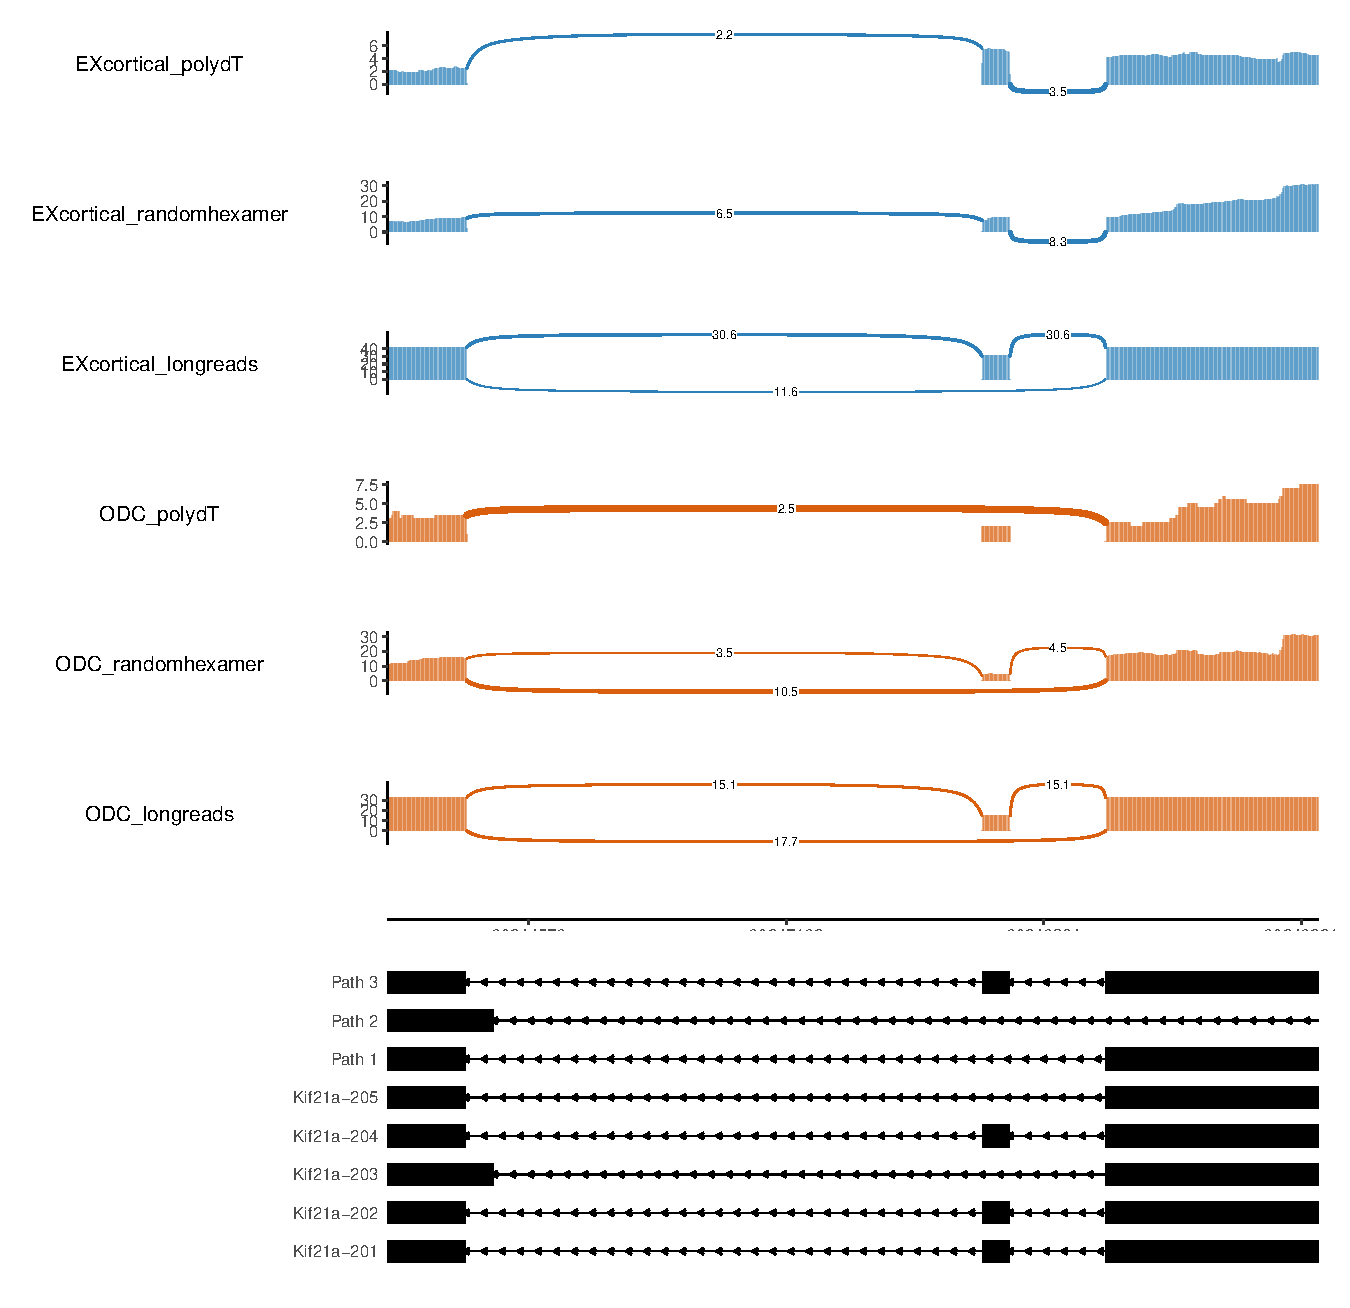
\includegraphics[width=1.15\textwidth,height=0.4\textheight,keepaspectratio]{figures/sashimi_Kif21a_B3.pdf}}\\
(b)
\caption{Kif21a block 3, cortical excitatory neurons against oligodendrocytes. Panels as in Figure~\ref{fig:pkn2}.}
\label{fig:kif21a}
\end{figure}

\begin{figure}[p]
\centering
\makebox[\textwidth][c]{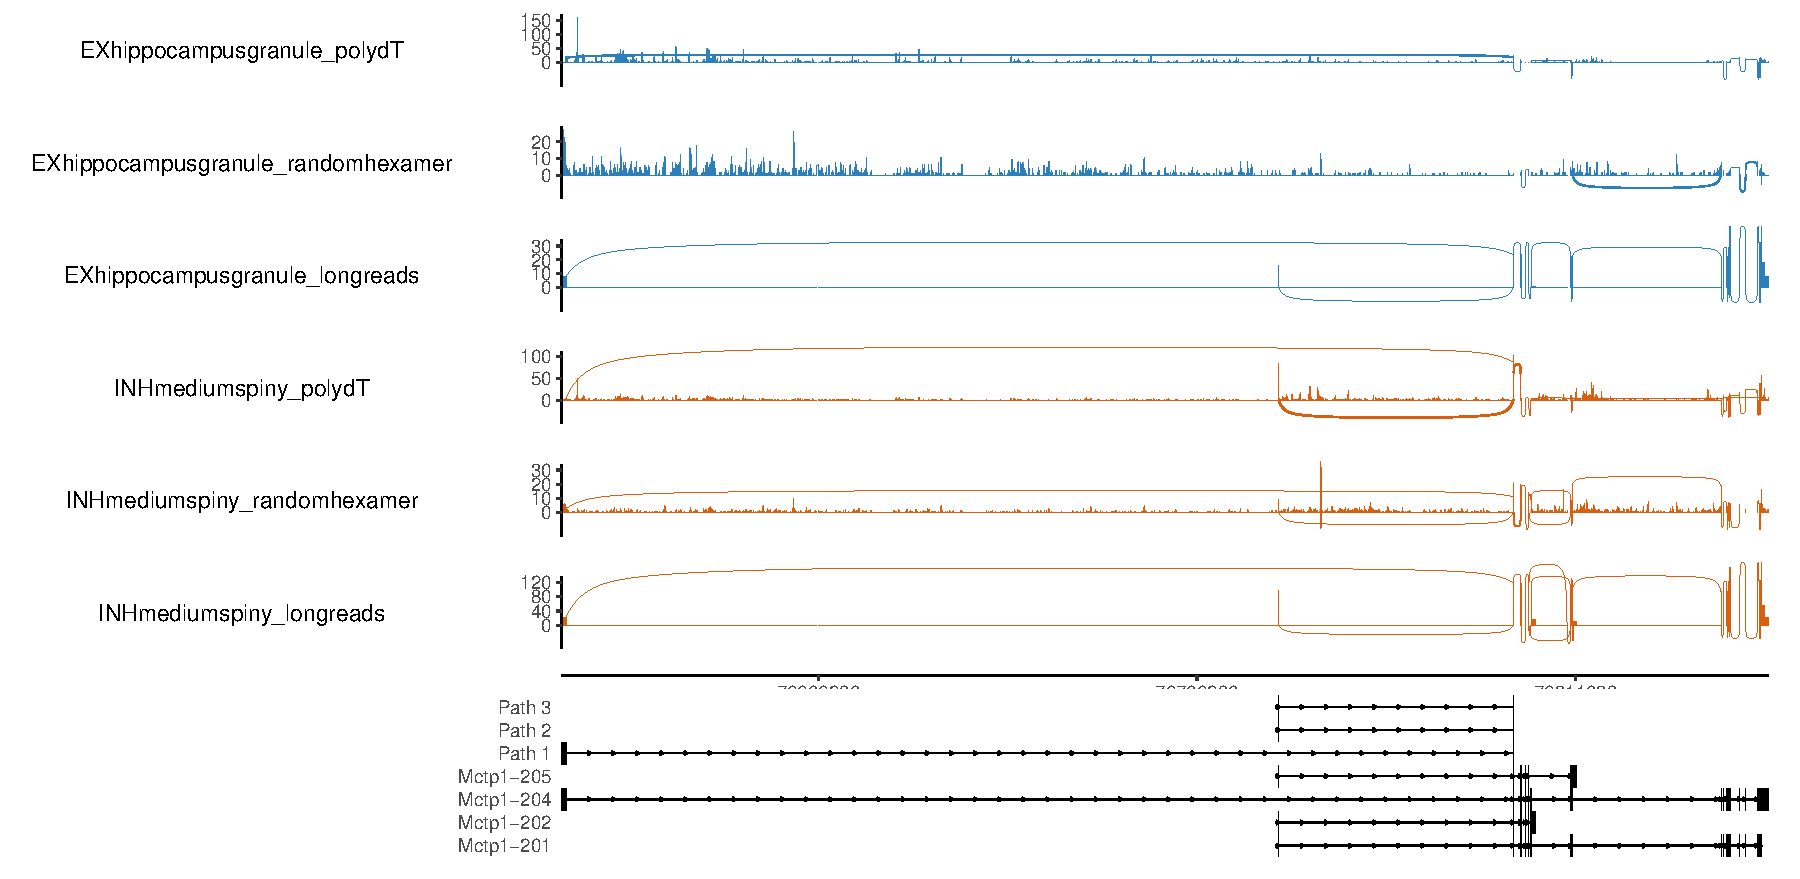
\includegraphics[width=1.15\textwidth,height=0.4\textheight,keepaspectratio]{figures/sashimi_Mctp1_B1_gene.pdf}}\\
(a)\\[4pt]
\makebox[\textwidth][c]{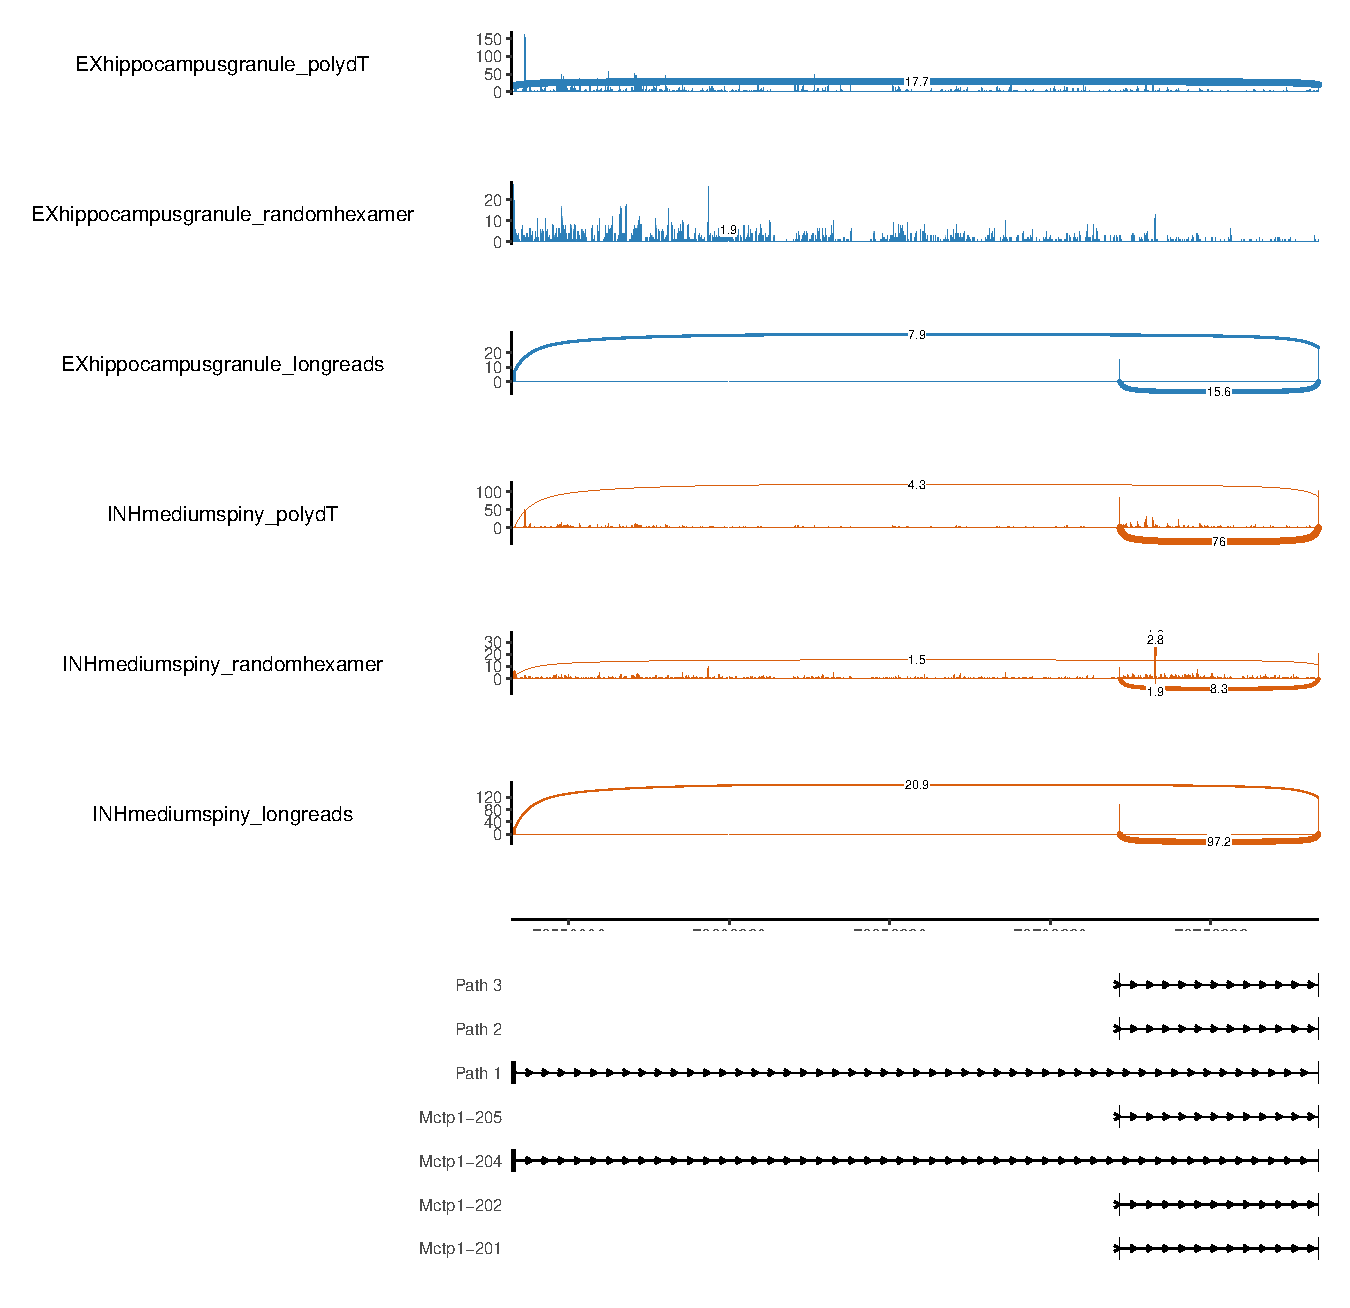
\includegraphics[width=1.15\textwidth,height=0.4\textheight,keepaspectratio]{figures/sashimi_Mctp1_B1.pdf}}\\
(b)
\caption{Mctp1 block 1, dentate gyrus granule neurons against medium spiny neurons, a terminal block tested on junction-spanning molecules. Panels as in Figure~\ref{fig:pkn2}.}
\label{fig:mctp1}
\end{figure}

\begin{figure}[p]
\centering
\begin{minipage}[t]{0.49\textwidth}\centering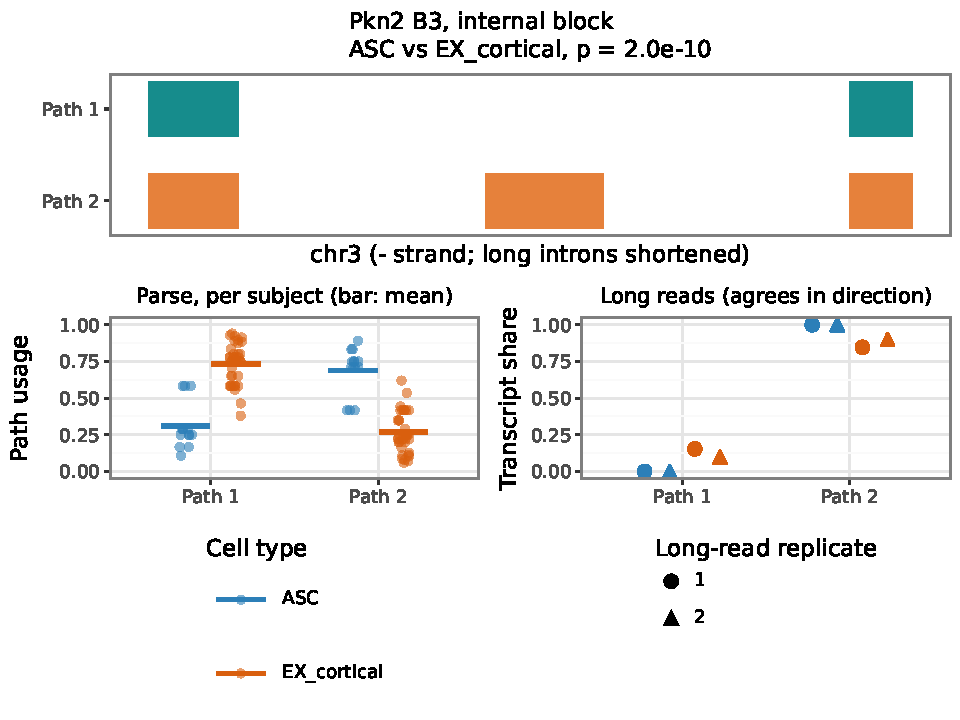
\includegraphics[width=\textwidth]{figures/example_Pkn2_B3.pdf}\\(a)\end{minipage}\hfill
\begin{minipage}[t]{0.49\textwidth}\centering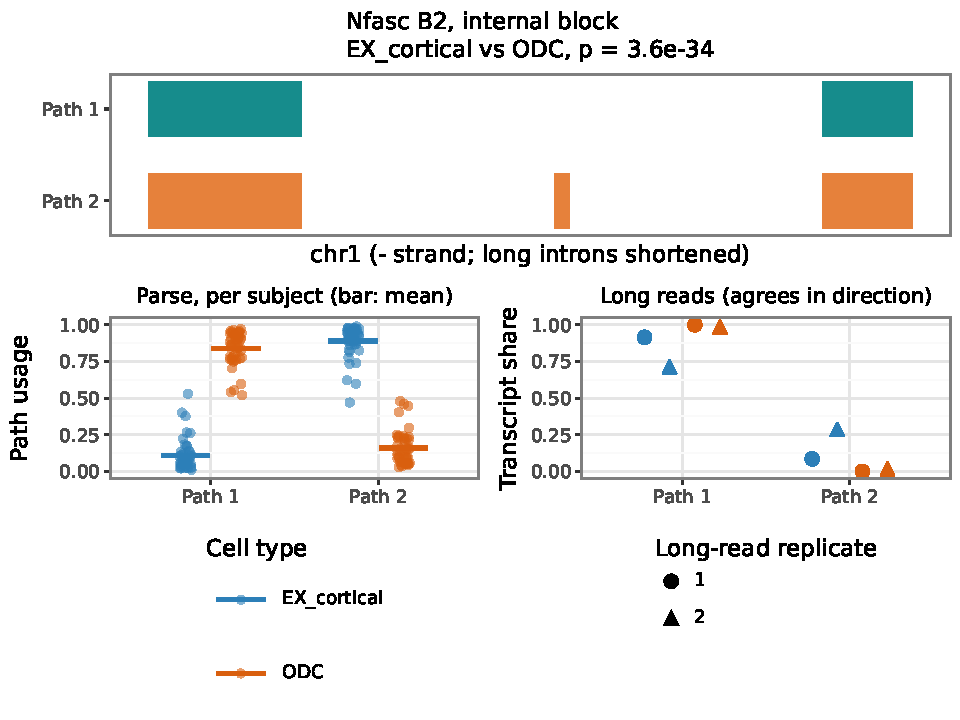
\includegraphics[width=\textwidth]{figures/example_Nfasc_B2.pdf}\\(b)\end{minipage}\\[6pt]
\begin{minipage}[t]{0.49\textwidth}\centering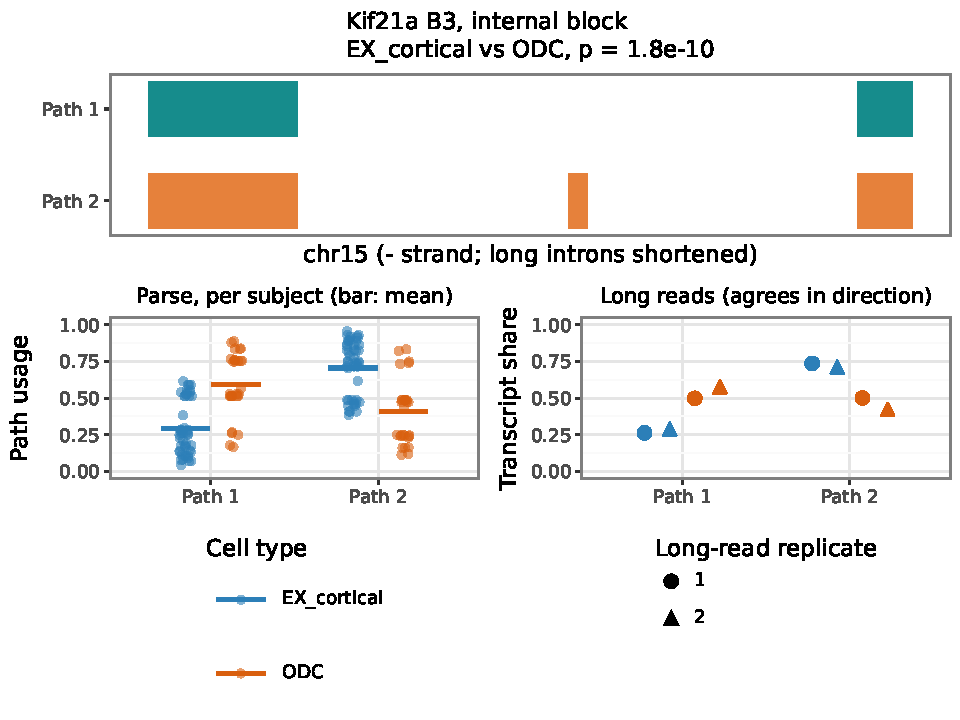
\includegraphics[width=\textwidth]{figures/example_Kif21a_B3.pdf}\\(c)\end{minipage}\hfill
\begin{minipage}[t]{0.49\textwidth}\centering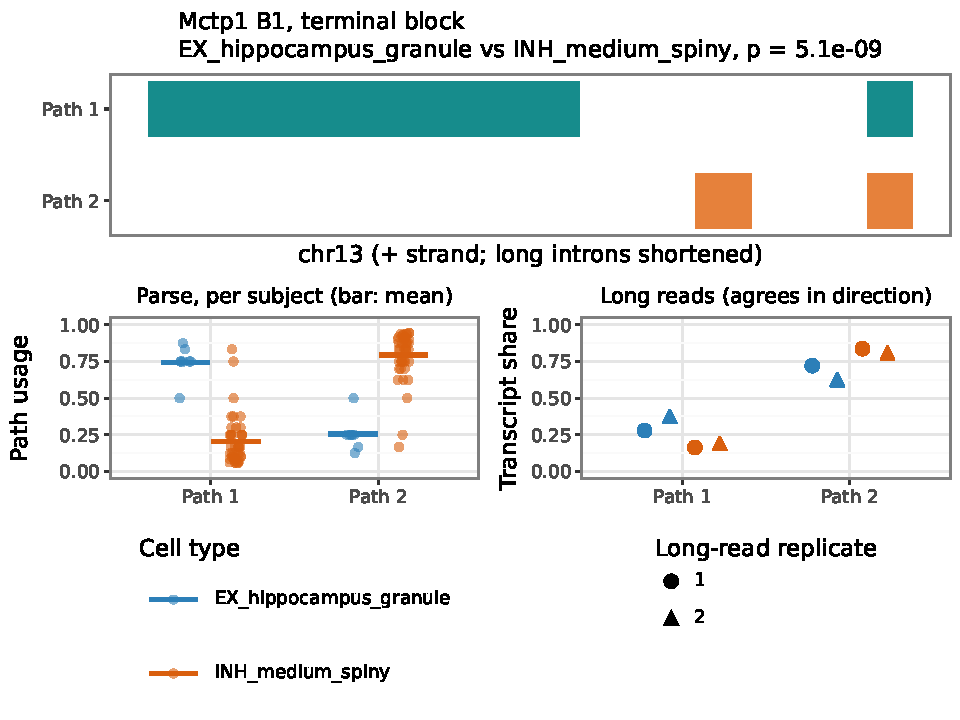
\includegraphics[width=\textwidth]{figures/example_Mctp1_B1.pdf}\\(d)\end{minipage}\\[6pt]
\caption{Path usage in the four examples: (a) Pkn2, (b) Nfasc, (c) Kif21a, (d) Mctp1. In each panel, top, the tested paths, numbered as in the sashimi plots (introns longer than 300 bases shortened; merged paths are drawn by their first member); bottom left, the path usage of each subject in the Parse data with the mean over subjects (bars); bottom right, the transcript share of each path in the two long-read replicates.}
\label{fig:usage}
\end{figure}

\section{Implementation}

The alignment kernel exists in two implementations with identical output, a numba implementation in the Python package and a Rust library called through a C interface. The Rust library also reads the paired gzipped FASTQ files. Each mate is decompressed and parsed on its own thread ahead of alignment, read 1 is converted to 2-bit codes, and read 2 is reduced to the corrected barcode and UMI. A run of 345 million read pairs aligns to the 1{,}163 genes of an earlier target list in 45~min with 16 threads, and to all 33{,}755 multi-exon genes in 32--67~min with 18 threads, compared with 67~min for STARsolo on 12 threads over the whole genome. Read opportunities, the row integrals and the subject quadrature are compiled numba kernels. Against STARsolo alignments of 2 million reads (earlier target list), the targeted aligner reports 97.6\% of STAR's unique alignments in the target loci as unique, with identical junctions for 99.5\% of reads aligned uniquely by both, and gives the same block class for 99.7\% of reads entering a block. Molecule counts per block, class, subject, cell type and primer agree with those from STARsolo alignments to within 5\% (overlap of 0.95 of STAR's counts), and the class distributions within blocks differ by a mean total-variation distance of 0.005.

\clearpage
\appendix

\section{Differential intron retention}
\label{sec:ir}

Block tests do not test retention of a whole intron, since a path whose chain is the block window duplicates the precursor path and is removed (935 retained-intron tests remain, Table~\ref{tab:events}). Retention is therefore tested per annotated intron. In nuclei most intronic molecules are precursor RNA, so the retained fraction of an intron is compared with that of the other introns of its gene.

\subsection{Counts}

Introns are the junctions of the comprehensive GENCODE vM32 transcripts of the target genes. An intron is \emph{clean} if no exon boundary of any transcript, of any gene and on either strand, lies strictly inside it; clean introns are disjoint. For clean intron $i$, subject $u$ and cell type $c$, $r_{iuc}\in\mathbb N_0$ is the number of retained molecules, sense molecules with an unspliced read inside the intron at least 5 bases from both ends, and $n_{iuc}\in\mathbb N_0$ the number of spliced molecules, those with a junction equal to the intron. Molecules are distinct half-cell barcode and UMI pairs, and both primers are pooled. Poly(dT) priming at genomic A-runs inflates intronic coverage, intron-body poly(dT) molecules per position being 27.5-fold higher within 100 bases upstream of a sense A-run (at least 8 A in 10 bases) than more than 3 kb away, 3.4-fold at 200--300 bases and 2- to 2.7-fold up to 3 kb, against 1.2- to 1.9-fold for random-hexamer molecules. Poly(dT) intron-body molecules within 1 kb upstream of a sense A-run are removed. The gene baseline of row $(u,c)$ is $R_{iuc}=\sum_{j\neq i}r_{juc}$ and $N_{iuc}=\sum_{j\neq i}n_{juc}$, with $j$ over the other clean introns of the gene.

\subsection{Model and test}

A test is indexed by a clean intron $i$ and a cell-type pair $\{c_0,c_1\}$, with rows $(u,c)$, $c\in\{c_0,c_1\}$, that have $r_{iuc}+n_{iuc}\ge3$ and $R_{iuc}+N_{iuc}\ge3$; at least 4 subjects must have rows in both cell types. Dropping the index $i$, the model is the random-effects model of the block test (Section~\ref{sec:block}) with one path against the rest and exact rows, \[r_{uc}\mid\psi_{uc}\sim\operatorname{Binomial}(r_{uc}+n_{uc},\psi_{uc}),\qquad \psi_{uc}\mid v_u\sim\BetaDist\big(\kappa\mu_{uc},\kappa(1-\mu_{uc})\big),\qquad v_u\sim\mathcal N(0,\sigma^2),\] with \[\logit\mu_{uc}=\theta_0+\theta_1z_c+v_u+o_{uc},\qquad o_{uc}=\log\frac{R_{uc}+0.5}{N_{uc}+0.5},\] where $\psi_{uc}\in(0,1)$ is the retained fraction of the row, $z_c=\mathbf 1[c=c_1]$ and the offset $o_{uc}\in\mathbb R$ is fixed. $\theta_1$ is then the change in the intron's retention relative to its gene, and a change of the whole gene's unspliced fraction between cell types enters through $o_{uc}$. Integration, estimation, bounds and the convergence check are those of the block test, and the likelihood-ratio statistic $T$ compares fits with and without $\theta_1$.

\paragraph{Calibration.} In simulations of this model with $k$ subjects, $P(\chi^2_1>T)$ rejects 10--12\% of null tests at 0.05 for $k\le6$, and the signed root of $T$ on $t_{k-1}$ is conservative. On the data, the null is generated by refitting 15\% of the tests, chosen at random, with each subject's two cell-type labels exchanged with probability $1/2$. This null rejects 8--10\% at 0.05, 2--3\% at 0.01 and 0.2--0.6\% at 0.001 under $\chi^2_1$, at every number of subjects from 4 to more than 18. 15--27\% of null statistics are below $10^{-3}$, and above their 80th percentile they follow $\chi^2_1$ scaled by a constant. With $q_\alpha$ the upper-$\alpha$ quantile of the null statistics and $\chi^2_{1,\alpha}$ that of $\chi^2_1$, the scale is $\varrho=\frac13\sum_{\alpha\in\{0.05,0.01,0.001\}}q_\alpha/\chi^2_{1,\alpha}$, estimated in each cohort, and the p-value is $P(\chi^2_1>T/\varrho)$. $\varrho$ is 1.30 and 1.34 in the two halves and 1.34 in the full data. A scaled $t$ distribution fitted by maximum likelihood to the null signed roots matches the bulk of the null but has a heavier tail and leaves no discoveries.

\paragraph{Per-subject comparison.} As a simpler alternative, $x_{uc}=\log\{(r_{uc}+0.5)/(n_{uc}+0.5)\}-o_{uc}$ with variance $w_{uc}=\sum_{y\in\{r,n,R,N\}}(y_{uc}+0.5)^{-1}$ gives per-subject differences $d_u=x_{uc_1}-x_{uc_0}$ with variance $w_{uc_0}+w_{uc_1}$, combined over the $k$ subjects with both cell types by the DerSimonian--Laird random-effects mean, with the Hartung--Knapp variance (floored at the DerSimonian--Laird variance) and $t_{k-1}$.

\subsection{Evaluation}

Cerebellar granule neurons are left out of the evaluation. Relative to the median of the eight long-read cell types, their gene-wide log ratio of intron-body to spliced molecules is $-1.99$ with poly(dT) and $-2.07$ with random hexamers (astrocytes $-0.43$ and $-0.49$, other types within $\pm0.13$). At introns without retained short-read molecules a test with the gene offset takes the sign of this baseline difference, and in the 28 pairs these tests make up most of the top-ranked long-read-evaluable tests of the per-subject comparison below. The evaluation uses the 21 pairs of the other seven long-read cell types. Split replication is scored as in Section~\ref{sec:evaluation}, with intron p-values combined by Simes within a gene--cell-type pair and the pairs of a gene by Simes, on each method's own (gene, pair) keys. In the long-read data a molecule retains a clean intron when one of its exons contains the intron with 20 bases on each side, and splices it when one of its junctions equals the intron. The long-read effect is the difference of retained fractions between the cell types, and a test is evaluable if each cell type has at least 20 long-read molecules retaining or splicing the intron and either (i) at least 5 molecules in the two cell types retain it or (ii) the retained fractions differ by at least 0.05. Agreement is the fraction of the 100 top-ranked evaluable tests whose effect has the sign of the long-read effect. SUPPA2 retained-intron events $\mathrm{RI}{:}\mathrm{chr}{:}s_1{:}e_1\text{-}s_2{:}e_2$ (1-based) are mapped to the clean intron $[e_1,s_2-1)$, and MAJIQ, built with intron retention, to its intron edges; an intron in several local splice variants keeps its smallest p-value.

\begin{table}[ht]
\centering
\footnotesize
\setlength{\tabcolsep}{4pt}
\begin{tabular}{lrrrrr}
\toprule
Method & Genes & BH genes per half & Replicated & LR retained $\ge5$ & LR difference $\ge0.05$\\
\midrule
Beta-binomial, gene offset & 4{,}626 & 30, 26 & 10 & .61 (5{,}820) & .58 (516)\\
\quad pooled retained $\ge50$ & 4{,}146 & 34, 31 & 10 & .65 (637) & -- (95)\\
\quad rows by primer & 4{,}134 & 24, 14 & 8 & .54 (4{,}921) & .54 (423)\\
\quad random hexamer only & 3{,}813 & 15, 16 & 5 & .54 (2{,}279) & .57 (285)\\
Per-subject comparison & 4{,}626 & 7, 9 & 2 & .45 (5{,}820) & .81 (516)\\
\quad random hexamer only & 3{,}813 & 2, 2 & 0 & .56 (2{,}279) & .76 (285)\\
SUPPA2 & 198 & 0, 0 & 0 & .43 (657) & .57 (224)\\
Primer-aware SUPPA2 & 119 & 0, 1 & 0 & .45 (494) & .56 (184)\\
MAJIQ & 31 & 8, 20 & 6 & -- (69) & -- (22)\\
\bottomrule
\end{tabular}
\caption{Differential intron retention on the 21 long-read cell-type pairs without cerebellar granule neurons. Genes is the number of genes with a test in both halves, BH genes per half the genes with BH-adjusted Simes p at most 0.05 in each half, and Replicated the genes with BH-adjusted conjunction p at most 0.05. The last two columns give the fraction of the 100 top-ranked long-read-evaluable tests that agree with the long-read direction under the two evaluability rules (number evaluable in parentheses; -- when fewer than 100). The pooled retained filter keeps tests with at least 50 retained molecules over both cell types, without labels. Rows by primer split each row by primer, each with that primer's gene offset.}
\label{tab:ir}
\end{table}

Table~\ref{tab:ir} gives the results. The Beta-binomial test replicates 10 of 4{,}626 genes against 2 for the per-subject comparison, 0 for both forms of SUPPA2 and 6 of 31 for MAJIQ, which tests few introns. A label-blind filter on pooled retained molecules leaves replication unchanged, rows by primer lower $\varrho$ to 1.23--1.27 but leave fewer tests, and random-hexamer molecules alone halve replication. Long-read agreement of the top-ranked tests is between 0.54 and 0.65 for every Beta-binomial variant and does not favour one test, since the Beta-binomial leads under the retained-molecule rule and the per-subject comparison under the difference rule. Among tests with at least 10 retained short-read molecules and a long-read difference of at least 0.05 (201 tests), the pooled short-read changes in retained fraction, with or without the gene offset, agree with the long-read direction in 51--52\% of tests. With these data differential intron retention between cell types is underpowered, with few replicated genes and weak agreement between short-read and long-read retention changes of single introns.

\end{document}
